\documentclass[10pt,a4paper,oneside]{article}
\usepackage[left=2cm,right=2cm,top=2cm,bottom=2cm]{geometry}

../../global_color_scheme.tex
\usepackage[utf8]{inputenc}
\usepackage[english]{babel}
\usepackage{forloop}
\usepackage{amsmath}
\usepackage{amsfonts}
\usepackage{amssymb}
\usepackage{gensymb}
\usepackage{graphicx}
\usepackage{tikz}
\usetikzlibrary{arrows,automata,shapes}
\usepackage[siunitx]{circuitikz}

\usepackage[colorlinks=true,linkcolor=blue,urlcolor=black,bookmarksopen=true]{hyperref}
\usepackage{bookmark}
\usepackage{hyperref}
\usepackage{sepfootnotes}

\usepackage[digital,srcmeas]{circdia}

\usepackage{float}
\floatstyle{boxed} 
\restylefloat{figure}

\title{Libre Silicon process specification}
\date{\today} 
\author{David Lanzendörfer}
\makeindex

\newcounter{ct}
\def\CrossSectionOnly{0.3}
\def\CrossAndTopSection{0.2}
\def\CrossAndTopSectionBig{0.3}
\def\VLSILayout{0.4}

\setlength{\parindent}{0pt} % get rid of annoying indents

\begin{document}
\maketitle

\begin{abstract}
	Copyright © 2017 LANCEVILLE TECHNOLOGY GROUP CO., LIMITED. All rights reserved. \\

	This process is licensed under the Libre Silicon public license; you can redistribute it and/or modify it under the terms of the Libre Silicon public license
	as published by the Libre Silicon alliance, either version 1 of the License, or (at your option) any later version.

	This design is distributed in the hope that it will be useful, but WITHOUT ANY WARRANTY; without even the implied warranty of MERCHANTABILITY or FITNESS FOR A PARTICULAR PURPOSE.
	See the Libre Silicon Public License for more details. \\

	This is the specification of the free silicon manufacturing standard for manufacturing the LibreSilicon standard logic cells\footnote{https://github.com/chipforge/StdCellLib} and related free technology nodes from the LibreSilicon project.
\end{abstract}

\newpage
\tableofcontents
\newpage
\section{CMOS in a nutshell}
This basic initial project is dedicated to the CMOS Technology only and for this reason two types of metal–oxide–semiconductor field-effect transistors (MOSFET) are required.

Historicaly, the first chips with MOSFETs on the mass market were p-channel MOSFETs in enhancement-mode.

\begin{center}
	\begin{figure}[h]
		\begin{center}
			\begin{circuitdiagram}{20}{20}
				\power{15}{18.5}{U}{}  % power above pmos
				\wire{15}{18}{15}{16}   % wire above pmos
				\trans{penh}{13}{14}{R}{}{} % pmos -> right
				\Voltarrow{14}{18}{10}{16}{u}{$-V_{GS}$}
				\wire{15}{12}{15}{8}   % wire below pmos
				\resis{15}{5}{V}{$R_D$}{}  % resistor on drain
				\wire{15}{1}{15}{2}   % wire below pmos
				\ground{15}{0.5}{D}  % ground below resistor
				\othersrc[\sigsym{-rec}]{o}{5.5}{15.5}{H}{}{signal}
				\pin{9.5}{15.5}{R}{}	% pin in
				\ground{2.5}{0.5}{D}  % ground below signal source
				\wire{2.5}{1}{2.5}{15.5}   % wire below signal
				\junct{15}{10}   % dot
				\wire{15}{10}{16}{10}   % wire before out
				\pin{17}{10}{R}{out}	% pin out
			\end{circuitdiagram}
		\end{center}
		\caption{enhancement-mode PMOS transistor use-case}
	\end{figure}
\end{center}

The sectional view of a PMOS transistor in silicon is being shown below
\begin{center}
	\begin{figure}[h]
		\begin{center}
			\begin{tikzpicture}[node distance = 3cm, auto, thick,scale=0.5, every node/.style={transform shape}]
				% substrate
				\fill[YellowOrange] (0,0) rectangle (10,2);
				\node at (2,0.5) {Si (p-type)};

				% n-well
				\fill[Goldenrod] (1.25,0.75) rectangle (8.25,2);
				\node at (5.75,1) {N-Well};

				% body
				\fill[ProcessBlue] (1.5,1) rectangle (3,2);
				\node at (2,1.5) {n+};
				% source
				\fill[RedOrange] (3.5,1) rectangle (5,2);
				\node at (4,1.5) {p+};
				% drain
				\fill[RedOrange] (6.5,1) rectangle (8,2);
				\node at (7,1.5) {p+};
				%% gate:
				% gate oxide
				\fill[LightGray] (4.8,2) rectangle (6.7,2.1);
				% gate poly
				\fill[BrickRed] (4.8,2.1) rectangle (6.7,2.2);

				% metals ground
				\fill[DarkDarkGray] (2,2) rectangle (2.5,3);
				\fill[DarkDarkGray] (4,2) rectangle (4.5,3);
				\fill[DarkDarkGray] (1,3) rectangle (4.5,3.2); % connection pad GND

				\fill[DarkDarkGray] (5.5,2.2) rectangle (6,3);
				\fill[DarkDarkGray] (5.3,3) rectangle (6.2,3.2); % connection pad VG

				\fill[DarkDarkGray] (7,2) rectangle (7.5,3);
				\fill[DarkDarkGray] (6.8,3) rectangle (7.7,3.2); % connection pad VDD

				% isolation oxides:
				\fill[NormalGray] (1,2) rectangle (2,3);
				\fill[NormalGray] (2.5,2) rectangle (4,3);
				\fill[NormalGray] (4.5,2) rectangle (4.8,3);
				\fill[NormalGray] (4.8,2.2) rectangle (5.5,3);
				\fill[NormalGray] (6,2.2) rectangle (6.7,3);
				\fill[NormalGray] (6.7,2) rectangle (7,3);
				\fill[NormalGray] (7.5,2) rectangle (8.5,3);

				\node at (1.5,3.5) {Source};
				\node at (5.5,3.4) {Gate};
				\node at (7.5,3.4) {Drain};

				%field oxides:
				\fill[DarkGray] (0,2) rectangle (1,4);
				\fill[DarkGray] (8.5,2) rectangle (10,4);
				\fill[RedOrange] (0,1.5) rectangle (1,2);
				\node at (0.5,1.75) {p+};
				\fill[RedOrange] (8.5,1.5) rectangle (10,2);
				\node at (9.5,1.75) {p+};
			\end{tikzpicture}
		\end{center}
		\caption{Sectional view of a PMOS transistor}
	\end{figure}
\end{center}

Historicaly later, faster chips with MOSFETs on the mass market were marked as n-channel MOSFETs in enhancement mode also.

\begin{center}
	\begin{figure}[h]
		\begin{center}
			\begin{circuitdiagram}{20}{20}
				\power{15}{18.5}{U}{}  % power above resistor
				\wire{15}{17}{15}{18}   % wire above resistor
				\resis{15}{14}{V}{$R_D$}{}  % resistor on drain
				\wire{15}{11}{15}{8}   % wire between resistor and nmos
				\trans{nenh}{13}{6}{R}{}{} % nmos -> right
				\Voltarrow{10}{4}{14}{1}{d}{$+V_{GS}$}
				\wire{15}{1}{15}{4}   % wire below nmos
				\ground{15}{0.5}{D}  % ground below nmos
				\othersrc[\sigsym{rec}]{o}{5.5}{4.5}{H}{}{signal}
				\pin{9.5}{4.5}{R}{}	% pin in
				\ground{2.5}{0.5}{D}  % ground below signal source
				\wire{2.5}{1}{2.5}{4.5}   % wire below signal
				\junct{15}{10}   % dot
				\wire{15}{10}{16}{10}   % wire before out
				\pin{17}{10}{R}{out}	% pin out
			\end{circuitdiagram}
		\end{center}
		\caption{enhancement-mode NMOS transistor use-case}
	\end{figure}
\end{center}

The sectional view of a NMOS transistor in silicon is being shown here also.
\begin{center}
	\begin{figure}[h]
		\begin{center}
			\begin{tikzpicture}[node distance = 3cm, auto, thick,scale=0.5, every node/.style={transform shape}]
				% substrate
				\fill[YellowOrange] (0,0) rectangle (10,2);
				\node at (2,0.5) {Si (p-type)};
				% body
				\fill[RedOrange] (1.5,1) rectangle (3,2);
				\node at (2,1.5) {p+};
				% source
				\fill[ProcessBlue] (3.5,1) rectangle (5,2);
				\node at (4,1.5) {n+};
				% drain
				\fill[ProcessBlue] (6.5,1) rectangle (8,2);
				\node at (7,1.5) {n+};
				%% gate:
				% gate oxide
				\fill[LightGray] (4.8,2) rectangle (6.7,2.1);
				% gate poly
				\fill[BrickRed] (4.8,2.1) rectangle (6.7,2.2);
				% metals ground
				\fill[DarkDarkGray] (2,2) rectangle (2.5,3);
				\fill[DarkDarkGray] (4,2) rectangle (4.5,3);
				\fill[DarkDarkGray] (1,3) rectangle (4.5,3.2); % connection pad GND

				\fill[DarkDarkGray] (5.5,2.2) rectangle (6,3);
				\fill[DarkDarkGray] (5.3,3) rectangle (6.2,3.2); % connection pad VG

				\fill[DarkDarkGray] (7,2) rectangle (7.5,3);
				\fill[DarkDarkGray] (6.8,3) rectangle (7.7,3.2); % connection pad VDD

				% isolation oxides:
				\fill[NormalGray] (1,2) rectangle (2,3);
				\fill[NormalGray] (2.5,2) rectangle (4,3);
				\fill[NormalGray] (4.5,2) rectangle (4.8,3);
				\fill[NormalGray] (4.8,2.2) rectangle (5.5,3);
				\fill[NormalGray] (6,2.2) rectangle (6.7,3);
				\fill[NormalGray] (6.7,2) rectangle (7,3);
				\fill[NormalGray] (7.5,2) rectangle (8.5,3);

				%field oxides:
				\fill[DarkGray] (0,2) rectangle (1,4);
				\fill[DarkGray] (8.5,2) rectangle (10,4);
				\fill[RedOrange] (0,1.5) rectangle (1,2);
				\node at (0.5,1.75) {p+};
				\fill[RedOrange] (8.5,1.5) rectangle (10,2);
				\node at (9.5,1.75) {p+};

				\node at (1.5,3.5) {Source};
				\node at (5.5,3.4) {Gate};
				\node at (7.5,3.4) {Drain};
			\end{tikzpicture}
		\end{center}
		\caption{Sectional view of a NMOS transistor}
	\end{figure}
\end{center}

Both technologies, the older NMOS as the newer PMOS, have the same disadvantage. Every time, the transistor is switched on, the current between Drain and Source of the transistor is limited by the Resistor on Drain only. Higher currents here meaning also higher power consumption for the chip where the transistors are integrated also. If the transistors are switched off, now currents flows between Drain and Source anymore, the power consumption of the chip also goes low.
Et violà, the US-Patent with Number 3356858\footnote{https://www.google.com/patents/US3356858} changed the world and combines both technologies to the new complementary metal-oxide-semiconductor (CMOS) technology. Instead of every transistor is working against a weak resistor, the transistor works against a complementary switched-off transistor. With the Eyes of our antecessor CMOS doubles the transistor count, but contemporary chips all are build in CMOS.

\begin{center}
	\begin{figure}[h]
		\begin{center}
			\begin{circuitdiagram}{20}{20}
				\power{15}{18.5}{U}{}  % power above pmos 
				\wire{15}{16}{15}{18}   % wire above pmos
				\trans{penh}{13}{14}{R}{}{} % pmos -> right
				\Voltarrow{14}{18}{10}{16}{u}{$-V_{GS}$}
				\wire{15}{8}{15}{12}   % wire between pmos and nmos
				\trans{nenh}{13}{6}{R}{}{} % nmos -> right
				\Voltarrow{10}{4}{14}{1}{d}{$+V_{GS}$}
				\wire{15}{1}{15}{4}   % wire below nmos
				\ground{15}{0.5}{D}  % ground below nmos
				\othersrc[\sigsym{rec}]{o}{5}{10}{H}{}{signal}
				\pin{9}{10}{R}{}	% pin in
				\wire{9.5}{10}{10}{10}   % wire before gates
				\wire{10}{15.5}{10}{4.5}   % wire between gates
				\junct{10}{10}   % dot
				\ground{2}{0.5}{D}  % ground below signal source
				\wire{2}{1}{2}{10}   % wire below signal
				\junct{15}{10}   % dot
				\wire{15}{10}{16}{10}   % wire before out
				\pin{17}{10}{R}{out}	% pin out
			\end{circuitdiagram}
		\end{center}
		\caption{complementary PMOS and NMOS transistor couple use-case}
	\end{figure}
\end{center}

Below the sectional view of the inverter circuitry can be seen.
For the run through of this process we will use this cross section diagram as reference.
\begin{center}
	\begin{figure}[h]
		\begin{center}
			\begin{tikzpicture}[node distance = 3cm, auto, thick,scale=0.5, every node/.style={transform shape}]
				% substrate
				\fill[YellowOrange] (0,0) rectangle (20,2);
				\node at (2,0.5) {Si (p-type)};
				% n-well
				\fill[Goldenrod] (1.25,0.75) rectangle (8.25,2);
				\node at (5.75,1) {N-Well};
				% body
				\fill[ProcessBlue] (1.5,1) rectangle (3,2);
				\node at (2,1.5) {n+};
				% source
				\fill[RedOrange] (3.5,1) rectangle (5,2);
				\node at (4,1.5) {p+};
				% drain
				\fill[RedOrange] (6.5,1) rectangle (8,2);
				\node at (7,1.5) {p+};
				%% gate:
				% gate oxide
				\fill[LightGray] (4.8,2) rectangle (6.7,2.1);
				% gate poly
				\fill[BrickRed] (4.8,2.1) rectangle (6.7,2.2);
				% isolation oxides:
				\fill[NormalGray] (1,2) rectangle (2,3);
				\fill[NormalGray] (2.5,2) rectangle (4,3);
				\fill[NormalGray] (4.5,2) rectangle (4.8,3);
				\fill[NormalGray] (4.8,2.2) rectangle (5.5,3);
				\fill[NormalGray] (6,2.2) rectangle (6.7,3);
				\fill[NormalGray] (6.7,2) rectangle (7,3);
				\fill[NormalGray] (7.5,2) rectangle (8.5,3);

				%field oxides:
				\fill[DarkGray] (0,2) rectangle (1,4);
				\fill[DarkGray] (8.5,2) rectangle (11.5,4);
				\fill[DarkGray] (19,2) rectangle (20,4);

				\fill[RedOrange] (0,1.5) rectangle (1,2);
				\fill[RedOrange] (8.5,1.5) rectangle (11.5,2);
				\fill[RedOrange] (19,1.5) rectangle (20,2);

				\node at (0.5,1.75) {p+};
				\node at (9.5,1.75) {p+};
				\node at (19.5,1.75) {p+};

				%%% nmos:
				% body
				\fill[RedOrange] (17,1) rectangle (18.5,2);
				\node at (18,1.5) {p+};
				% source
				\fill[ProcessBlue] (15,1) rectangle (16.5,2);
				\node at (16,1.5) {n+};
				% drain
				\fill[ProcessBlue] (12,1) rectangle (13.5,2);
				\node at (13,1.5) {n+};

				%% gate:
				% gate oxide
				\fill[LightGray] (13.3,2) rectangle (15.2,2.1);
				% gate poly
				\fill[BrickRed] (13.3,2.1) rectangle (15.2,2.2);

				% metals
				\fill[DarkDarkGray] (17.5,2) rectangle (18,3);
				\fill[DarkDarkGray] (15.5,2) rectangle (16,3);
				\fill[DarkDarkGray] (15.5,3) rectangle (19,3.2); % connection pad GND

				\fill[DarkDarkGray] (14,2.2) rectangle (14.5,3);
				\fill[DarkDarkGray] (13.8,3) rectangle (14.7,3.2); % connection pad VG

				\fill[DarkDarkGray] (12.5,2) rectangle (13,3);
				\fill[DarkDarkGray] (12.3,3) rectangle (13.2,3.2); % connection pad VDD

				\fill[DarkDarkGray] (2,2) rectangle (2.5,3);
				\fill[DarkDarkGray] (4,2) rectangle (4.5,3);
				\fill[DarkDarkGray] (1,3) rectangle (4.5,3.2); % connection pad GND

				\fill[DarkDarkGray] (5.5,2.2) rectangle (6,3);
				\fill[DarkDarkGray] (5.3,3) rectangle (6.2,3.2); % connection pad VG

				\fill[DarkDarkGray] (7,2) rectangle (7.5,3);
				\fill[DarkDarkGray] (6.8,3) rectangle (7.7,3.2); % connection pad VDD

				% isolation oxides:
				\fill[NormalGray] (18,2) rectangle (19,3);
				\fill[NormalGray] (16,2) rectangle (17.5,3);
				\fill[NormalGray] (15.2,2) rectangle (15.5,3);
				\fill[NormalGray] (14.5,2.2) rectangle (15.2,3);
				\fill[NormalGray] (13.3,2.2) rectangle (14,3);
				\fill[NormalGray] (13,2) rectangle (13.3,3);
				\fill[NormalGray] (11.5,2) rectangle (12.5,3);

				\node at (1.5,3.5) {VDD};
				\node at (16.5,3.5) {Ground};
				\node at (5.5,3.4) {Input};
				\node at (14,3.4) {Input};
				\node at (7,3.4) {Output};
				\node at (12.5,3.4) {Output};

				\node at (0.5,4.2) {Field oxide};
				\node at (9.5,4.2) {Field oxide};
				\node at (19.5,4.2) {Field oxide};
			\end{tikzpicture}
		\end{center}
		\caption{Sectional view of a NMOS-PMOS transistor circuit}
	\end{figure}
\end{center}

\newpage
\section{Physics}
\subsection{Infusion}
The redistribution process depends on the ratio of the solubility of the doping material in silicon and SiO$ _2$. At the Si/SiO$ _2$ interface the dopants are redistributed by segregation until the ratio of their concentration at the interface is the same as the ratio of their solubility in both materials. The ratio of dopant solubility is expressed by the segregation coefficient $m$ which is

\begin{equation}
\displaystyle m = \frac{
	\mathrm{solubility\ in\ silicon}
	}{
	\mathrm{solubility\ in\ SiO_2}
	}
\end{equation}

As listed in \autoref{table_diffusion_coeff} below there are dopant species which solubilize better in SiO$ _2$ than in silicon ($ m < 1$) and species which have a reversed behavior ($ m > 1$).
In case of $ m < 1$, as for Boron, the dopant concentration is enhanced at the SiO$ _2$ side, whereas beneath the interface, there is a dopant depletion at the silicon surface.
For reversed solubility ratios ($ m > 1$, like Phosphorus), only few dopant atoms penetrate the interface.
In order to obtain the by $ m$ determined concentration ratio at the interface, dopant atoms from deeper silicon zones diffuse back to the surface zone.
Therefore, the dopant concentration at the silicon surface is enhanced, as illustrated in \autoref{graph_figure}b.
In \autoref{graph_figure} $ C_c$ denotes the dopant concentration in the silicon surface zone before oxidation. $ x$ is the distance from the silicon surface.

\begin{center}
	\begin{figure}[h]
		\begin{center}
			\includegraphics[width=0.75\linewidth]{img349.png}
		\end{center}
		\caption{Schematic illustration of dopant redistribution}
		\label{graph_figure}
	\end{figure}
	\begin{table}[h]
		\begin{tabular}{|c|c|c|c|c|c|}
			\hline
			Dopant species &
			Boron &
			Phosphor &
			Antimon &
			Arsen &
			Gallium \\
			\hline
			$m$ &
			0.1-0.3 &
			10 &
			10 &
			10 &
			20 \\
			\hline
		\end{tabular}
		\caption{Segregation coefficients $m$ for important dopant species in silicon}
		\label{table_diffusion_coeff}
	\end{table}
\end{center}
\newpage
\section{MOS Capacitance}
\url{https://ecee.colorado.edu/~bart/book/book/chapter6/ch6_3.htm}

\subsection{Threshold voltage ($V_T$)}
The formula for calculating the threshold voltage of a MOS device is the following:
\begin{equation}
V_T = V_{t-mos} + V_{FB}
\end{equation}
where $V_{t-mos}$ is the ideal threshold voltage of an ideal MOS capacitor and $V_{FB}$ is what is termed flat-band voltage and $V_{t-mos}$ is the threshold.
The MOS threshold voltage, $V_{t-mos}$ is calculated by considering the MOS capacitor structure that form the gate of the MOS transistor.
The ideal threshold voltage may be expressed as:
\begin{equation}
V_{t-mos}=2 \phi_F + \frac{Q_b}{C_{ox}}
\end{equation}
with
\begin{equation}
Q_b
=
\sqrt{2 \epsilon_{Si} q N_A ( 2 \phi_F + V_{SB}) }
\end{equation}
\begin{equation}
\phi_F
=
V_{th} ln\left(\frac{N_A}{N_i}\right)
=
\frac{k T}{q} ln\left(\frac{N_A}{N_i}\right)
\end{equation}
where $C_{ox}$ is the oxide capacitance and $Q_b$ which is called the bulk charge term and $V_{th}$ is the thermal voltage.\footnote{\url{https://en.wikipedia.org/wiki/Boltzmann_constant\#Role_in_semiconductor_physics:_the_thermal_voltage}}

Because we put source and bulk onto the same potential in our CMOS circuit as shown in \autoref{process_design} we can put $V_{BS}=0$ which results in the following new equation for $Q_B$:
\begin{equation}
V_{BS}=0
\Rightarrow
Q_b
=
\sqrt{2 \epsilon_{Si} q N_A 2 \phi_F }
=
2 \sqrt{\epsilon_{Si} q N_A \phi_F }
\end{equation}

 $V_{FB}$, is given by:
\begin{equation}
V_{FB}
=
\phi_{MS}-\frac{Q_f}{C_{ox}}-\frac{1}{C_{ox}}\int_{0}^{t_{ox}}\frac{x}{x_{ox}}\rho(x) dx
\end{equation}
We assume the oxide doesn't contain any charge, which makes the equation fall together into
\begin{equation}
\rho(x)=0
\Rightarrow
V_{FB}
=
\phi_{MS}-\frac{Q_f}{C_{ox}}
\end{equation}
with
\begin{equation}
\phi_{MS}
=
\phi_{M} - \phi_{S}
=
\phi_{M} -  \left( \frac{E_g}{2 q} + \phi_F \right)
=
\phi_{M} - \frac{E_g}{2 q} - \phi_F
\end{equation}

We now can put the equation together:
\begin{equation}
V_T = V_{t-mos} + V_{FB}
\end{equation}
\begin{equation}
V_{t-mos}=2 \phi_F + \frac{Q_b}{C_{ox}}
\Rightarrow
V_T = 2 \phi_F + \frac{Q_b}{C_{ox}} + V_{FB}
\end{equation}
\begin{equation}
V_{FB}
=
\phi_{MS}-\frac{Q_f}{C_{ox}}
\Rightarrow
V_T = 2 \phi_F + \frac{Q_b}{C_{ox}} + \phi_{MS}-\frac{Q_f}{C_{ox}}
\end{equation}
\begin{equation}
Q_b
=
2 \sqrt{\epsilon_{Si} q N_A \phi_F }
\Rightarrow
V_T = 2 \phi_F + \frac{2 \sqrt{\epsilon_{Si} q N_A \phi_F }}{C_{ox}} + \phi_{MS}-\frac{Q_f}{C_{ox}}
\end{equation}


\begin{equation}
\phi_{MS}
=
\phi_{M} - \frac{E_g}{2 q}-\phi_F
\Rightarrow
V_T = 2 \phi_F + \frac{2 \sqrt{\epsilon_{Si} q N_A \phi_F }}{C_{ox}} + \phi_{M} - \frac{E_g}{2 q}-\phi_F -\frac{Q_f}{C_{ox}}
\end{equation}
\begin{equation}
\Rightarrow
V_T = \phi_F + \frac{2 \sqrt{\epsilon_{Si} q N_A \phi_F }-Q_f}{C_{ox}} + \phi_{M} - \frac{E_g}{2 q}
\end{equation}


\begin{equation}
\phi_F
=
\frac{k T}{q} ln\left(\frac{N_A}{N_i}\right)
\end{equation}
\begin{equation}
\Rightarrow
V_T = \frac{k T}{q} ln\left(\frac{N_A}{N_i}\right) + \frac{2 \sqrt{\epsilon_{Si} q N_A \frac{k T}{q} ln\left(\frac{N_A}{N_i}\right) }-Q_f}{C_{ox}} + \phi_{M} - \frac{E_g}{2 q}
\end{equation}
\begin{equation}
 \boxed{
\Rightarrow
V_T = \frac{k T}{q} ln\left(\frac{N_A}{N_i}\right) + \frac{2 \sqrt{\epsilon_{Si} N_A k T ln\left(\frac{N_A}{N_i}\right) }-Q_f}{C_{ox}} + \phi_{M} - \frac{E_g}{2 q}
}
\end{equation}


With the variables being the following:
\begin{itemize}
\item $N_A$ is the substrate doping (which in the case of our chosen basis substrate is approximately $9\times10^{14}cm^{-3}$ (see \autoref{process_overview}))
\item $N_i$ is the carrier concentration in intrinsic (undoped) silicon. $N_i$ is equal to $1.45 \times 10^{10} cm^{-3}$ at 300\degree K
\item $\phi_M = 4.1 V$ is the "work function" of our metal at the gate (multiplied with q) (Only Aluminum is practical for this process)
\item $E_g$ is the band gap energy of silicon: $\left(1.16-0.704 \times 10^{-3} \frac{T^2}{T+1108} \right)^5$
\item $C_{ox}$ is the oxide capacitance
\end{itemize}


\subsection{The substrate bias effect}
\section{Threshold voltage ($V_T$) adjustment}
At some point in the future this will be of very high relevance, because the lower the size of the transistors becomes, the higher the offset to $V_{Tp}$ and $V_{Tn}$ needs to be in order to stay on TTL 5V logic level, or at least compensate for the lowered voltages in order to reach the 3.3V CMOS logic levels.

Adjustment of the threshold voltage can be achieved by:
\begin{itemize}
\item A relatively small dose $N_I$ (units: ions/$cm^2$) of dopant atoms is implanted into the near-surface  region of the semiconductor.
\item When the MOS device is biased in depletion or inversion, the implanted dopants add to (or substract from) the depletion charge near the oxide-semiconductor interface
\end{itemize}

The formula to calculate the voltage offset is:
\begin{equation}
\Delta V_T = -\frac{q N_I}{C_{ox}} 
\left\{\begin{matrix}
N_I > 0\ for\ donor\ atoms\ (Phosporus/N) \\
N_I < 0\ for\ acceptor\ atoms\ (Boron/P)
\end{matrix}\right.
\end{equation}

\newpage
\section{Chemistry}
\subsection{Etching}
\subsubsection{Silicon dioxide}
A very "selective" chemical for SiO2 - i.e. does not etch silicon at all - is hydrofluoric acid (HF). If used directly such etchant has a too fast and aggresive action on the oxide, making very difficult the undercut and the linewidth control. For such reason, HF is universally used as a "buffered" solution, which can keep the etch rate low and constant, by moderating the PH level of the bath. This allows the etching time to be reliably correlated to the etching depth.

The industry standard buffered hydrofluoric acid solution (BHF) has the following formulation:

- 6 volumes of ammonium floride (NH4F, 40% solution) - 1 volume of HF.

This can be prepared, for example, by mixing 113 g of NH4F in 170 ml of H2O, and adding 28 ml of HF. The etch rate at room temperature can range from 1000 to 2500 Å/min. This depends on the actual density of the oxide which, as an amorphous layer, can have a more compact structure (if thermally grown in is oxygen) or less compact (if grown by CVD). The following etching reaction holds:

\begin{equation}
SiO_2 + 6HF \rightarrow H_2SiF_6 + H_2O
\end{equation}

where H2SiF6 is water soluble.

Sometimes the BHF is prepared and stored according to the formulation given above, but it is 7:1 diluited in water just before being used. This allows an even better control of the etching rate. It is good practice to use the diluited BHF only once and then discard it, in order to assure process repeatability. If a diluited BHF bath at 35°C is used, the etching rate for thermal oxide is around 800Å/min.

Another popular etching formulation is the P-etch:

60 volumes of H2O + 3 vol. of HF + 2 vol. of HNO3, that is: 300 ml of H2O + 15 ml of HF + 10 ml of HNO3.

The P-etch action is strongly dependent on oxide density, as it results from the growth technique. An example is reported in the literature\footnote{A. Pliskin, J.Vac.Sci Technol., vol. 14, p.1064, 1977}, indicating 120 Å/min for thermal oxide and 250-700 Å/min for sputtered oxide.

A slow etching bath is preferred for opening mask windows for a silicon substrate. However, the etching process could be used just for removing the oxide film from the whole surface. In this case the etching speed is not critical, and a fast solution can be used, such as HF diluited 1:10 in water. The etching time can be easily evaluated by visually inspecting the surface. Once the oxide film is removed, the metal-grey color of the silicon surface appears.

Sometimes a very light etch is required, for removing just a few atomic layers. This is the case of surface cleaning and decontamination. HF diluited 1 : 50 in water can be used. The etching speed will be around 70 Å / min. For example, a typical 50 Å "native" oxide on silicon can be removed with a 45 - 50 sec light etch.


\subsection{Growing silicon nitride}\label{chemistry_growing_nitride}
In order to grow a high quality layer of silicon nitride on top of a silicon wafer which is adapted to be patterned and to serve as a mask for diffusion or implantation of selected impurities, the wafer is being best put into a chamber evacuated to a pressure less than about 1 Torr and heated to between 650 and 900 \degree C;
A gaseous mixture comprising primarily ammonia and a silicon compound is being flooded into that chamber with a silicon compound flow rate of greater than approximately 12 cubic centimeters per minute and the ammonia and selected silicon compound having a ratio of relative concentrations in the range of 4:1 and 20:1.\footnote{\url{http://www.freepatentsonline.com/4395438.html}}
The growth rate will be around 50 Angstroms per minute.
That setup is called Low-Pressure Chemical Vapor Deposition (LPCVD), which is commonly available in basically any semiconductor manufacturing plant or laboratory.

\newpage
\section{Process design}
We need to optimize our process to be TTL compatible (5V logic levels) and at the same time being as fast and power efficient as possible.
In order to have a good propagation delay with a technology node of around $1\mu m$ we will have to have gates with up to four stacked MOS transistors.

Acceptable input signal voltages range from 0 volts to 0.8 volts for a low logic state, and 2 volts to 5 volts for a high logic state.
Acceptable output signal voltages shall range from 0 volts to 0.5 volts for a low logic state, and 2.7 volts to 5 volts for a high logic state\footnote{\url{https://www.allaboutcircuits.com/textbook/digital/chpt-3/logic-signal-voltage-levels}}

\begin{figure}[H]
	\centering
	\includegraphics[scale=0.5]{logic_levels.png}
	\caption{TTL logic levels}
	\label{TTL_logic_levels}
\end{figure}

As shown in \autoref{TTL_logic_levels} we have some margin to make our PMOS and NMOS transistors work with each other in order to form a CMOS circuit which is actually working without getting warm.

Or more clearly defined
\begin{equation}
V_{off} \leq 0.8V
\end{equation}
and
\begin{equation}
V_{on} \geq 2V
\end{equation}
which are limits, elementary to our design.

\begin{figure}[H]
	\centering
	\includegraphics[scale=0.5]{cmos_3v3.png}
	\caption{CMOS 3.3V logic levels}
	\label{CMOS_logic_levels}
\end{figure}

This means that we also will be compatible to CMOS logic level output pins since their ON/OFF levels are within our tolerance range\footnote{\url{https://learn.sparkfun.com/tutorials/logic-levels/33-v-cmos-logic-levels}} as it is shown in \autoref{CMOS_logic_levels}.
\input{process_design_requirements.tex}
\section{Substrate}

The Hong University of science and technology (short HKUST) provides us with two types of wafers.

\begin{itemize}
	\item Prime Grade Silicon Wafer, [100] N-type
	\begin{itemize}
		\item Front-side polished, backside etched
		\item Dopant: Phosphorus
		\item Thickness: $525 \mu m \pm 25 \mu m$
		\item Resistivity:4 to 7ohm-cm
		\item Growth Method: CZ
		\item Diameter: 100mm +/- 0.5 mm
		\item Primary  \& secondary flat locations: (In compliance with the SEMI)
			\begin{itemize}
				\item Carbon concentration<2.5 x e16 atm/cc
				\item Oxygen concentration < $9.0 \cdot 10^{17} \frac{atm}{cc}$
				\item $TTV < 10 \mu m$
				\item $TIR < 6 \mu m$
				\item $Bow/Warp < 40 \mu m$
			\end{itemize}
	\end{itemize}
	\item Prime Grade Silicon Wafer, [100] P-type
	\begin{itemize}
		\item Front-side polished, backside etched
		\item Dopant: Boron
		\item Thickness: $525 \mu m \pm 25 \mu m$
		\item Resistivity:15 to 25 ohm-cm
		\item Growth Method: CZ
		\item Diameter: 100mm +/- 0.5 mm
		\item Primary  \& secondary flat locations: (In compliance with the SEMI)
			\begin{itemize}
				\item Carbon concentration<2.5 x e16 atm/cc
				\item Oxygen concentration < $9.0 \cdot 10^{17} \frac{atm}{cc}$
				\item $TTV < 10 \mu m$
				\item $TIR < 6 \mu m$
				\item $Bow/Warp < 40 \mu m$
			\end{itemize}
	\end{itemize}
\end{itemize}

For this process the p-doped mono crystalline silicon substrate is being used, but forks and modifications will be very well possible based on a Graphene substrate or alike, still under the LSPL.
The starting material is a p-doped <100> oriented mono crystalline silicon wafer\\

\textbf{Reasons for using p-doped substrate}:\begin{itemize}
\item We can't use two different substrates for our design because in the design both PMOS and NMOS is present.
We have to choose which is more beneficial from fabrication point of view.
In general or say it's true that NMOS devices are always more in the Semiconductor Industry in comparison to PMOS devices.
For your reference-SRAM requires 6 transistors (4 NMOS, 2 PMOS).
\item Another reason for more number of NMOS is because of difference of mobility of electron and holes.
Electron mobility is almost twice of holes mobility and because of this ON-RESISTANCE of n-channel device is half of p-channel device with the same geometry and under the same operating conditions.
That means to achieve same impedance size of n-channel transistors is almost half of p-channel devices.
Same thing I can say in the different way that for same size of wafer, we can have more number of NMOS (means can perform more logical operation) in comparison to PMOS.
\item Since we only have the choice between P and N doped substrate, we use P doped substrate, because of the carrier mobility
\end{itemize}

Using the method from \autoref{r_l_nd_relation} we get a doping concentration between $8.76 \cdot 10^{14} \frac{1}{cm^3}$ and $5.23 \cdot 10^{14} \frac{1}{cm^3}$.
The average of this range is $N_B = \frac{8.76+5.23 }{2} \cdot 10^{14} \frac{1}{cm^3} \approx 7 \cdot 10^{14} \frac{1}{cm^3}$
\subsection{Isolation}
For the isolation (\autoref{sti})  in this design the STI approach is being chosen.
Shallow trench isolation (STI), also known as box isolation technique, is an integrated circuit feature which prevents electric current leakage between adjacent semiconductor device components.\footnote{\url{https://www.google.com/patents/US7985656}}
STI is generally used on CMOS process technology nodes of 250 nanometers and smaller.\\

\textbf{Reasons for using box isolation}:\begin{itemize}
\item We want to be forward compatible to future LibreSilicon nodes with a size of 100nm or smaller
\item It simplifies the construction of the gate and allows us to use Aluminum instead of Polysilicon for the gate contact
\end{itemize}

\subsection{Interconnect}
The interconnects and the gate electrode are being made using Aluminum which is a very commonly used material to do interconnects in low-frequency and low-resolution applications \\

\textbf{Reasons for using Aluminum}:\begin{itemize}
\item It's a well explored material for interconnect with a lot of literature on how to process it
\item Aluminum is easy to etch compared to copper
\item It isn't contaminating everything like copper does and doesn't require special separated setup for handling
\item The machines at HKUST can do CMP for copper only on 4 inch wafers which would limit us in wafer size
\end{itemize}

\begin{mdframed}[linewidth=2pt,linecolor=green]
As soon as we've got CMOS all figured out, we will tackle copper interconnect in release 2.0
\end{mdframed}
\subsection{MOS gate}
The wires and the MOS gates can be modeled as an RC low-pass filter, for that reason the time constant $\tau=RC$ is limiting the clock frequency of our CMOS circuitry.
However, we can't just make the gate ultra thin, because lowered capacity also creates lowered thresholds, which will be a very big problem, as soon as we go into the 100nm range and lower.

In \autoref{nmos_gate_dimensioning} we defined the capacity of the gate to be $C_{ox} \leq 305.7 \frac{nF}{cm^2}$ which leads to the oxide capacity-thickness constraint with the variables being:
\begin{itemize}
\item $\epsilon_0 = 8.85 \cdot 10^{-14}\frac{F}{cm}. $ is the electric permittivity in vacuum
\item $\epsilon_{ox} =3.9 \cdot \epsilon_0$ is the relative permittivity of silicon dioxide
\end{itemize}
and the constraint being for the oxide thickness which is only silicon dioxide for now
\begin{equation}
C_{ox}
=
\frac{\epsilon_{ox}}{t_{ox}}
\end{equation}
\begin{equation}
t_{ox}
=
\frac{\epsilon_{ox}}{C_{ox}}
\end{equation}

And with numbers we get
\begin{equation}
t_{ox}
=
\frac{3.9 \cdot 8.85 \cdot 10^{-14}\frac{F}{cm}}{305.7 \frac{nF}{cm^2}}
=
1.129 \cdot 10^{-6} cm
=
11.29nm
\end{equation}

That's still doable with a precision high enough when using dry oxidation and a temperature of 1000\degree Celsius.
\subsection{NMOS threshold}\label{nmos_gate_dimensioning}
First we take a look at the worst case of 4 stacked NMOS transistors, which is the highest stacking amount which will be possible in technologies relying on this process.

\input{process_design_graphics/schematic_AND4.tex}
As shown in  \autoref{TTL_logic_levels} our acceptable voltages for our CMOS "ON" state range from 2V to VDD (which typically is around $5V\pm0.25V$)

\begin{equation}
V_{on} \geq 2V
\end{equation}

Because there are four transistors dividing the voltage by being in series, the power supply voltage is being divided by the amount of transistors in series.
In order to match the threshold voltages of all of the transistors, which is needed for a working digital logic, the following equation need to be satisfied

\begin{equation}
V_{on} > 4 \cdot V_{Tn}
\end{equation}

Lets assume the worst case with

\begin{equation}
V_{on} = 2V
\end{equation}

Which leads to the required worst case threshold tolerance value

\begin{equation}
4 \cdot V_{Tn} < 2V
\Rightarrow
V_{Tn} < 500mV
\end{equation}
 
 Using the equation from \autoref{transistor_threshold_calculation} we can now set in this value and play around with the parameters.
 
 \begin{equation}
V_T= \frac{1.66 \cdot 10^{-7}}{C_{ox}}-0.094
\end{equation}

For safety reasons we take 10\% of the worst case as a error margin which leads us to the following new equation to solve
 \begin{equation}
V_T = 450mV
\end{equation}

This gives us the constraint of
\begin{equation}
0.45 V = \left( \frac{1.66 \cdot 10^{-7}}{C_{ox}}-0.094 \right) V
\end{equation}

We solve for the target capacity (in $\frac{F}{cm^2}$) which gives us the desired threshold voltage:
\begin{equation}
\Rightarrow
C_{ox}
=
3.057 \cdot {10}^{-7} \frac{F}{cm^2}
\end{equation}
\begin{equation}
\Rightarrow
C_{ox}
=
305.7 \frac{nF}{cm^2}
\end{equation}
\subsection{PMOS threshold}\label{pmos_dimensioning}
Now we take a look at the worst case of 4 stacked PMOS transistors, which is the highest stacking amount which will be possible in technologies relying on this process.
\input{process_design_graphics/schematic_OR4.tex}


With our $\phi_F$ for a doped n-well
\begin{equation}
\phi_F
=
V_{th} ln\left(\frac{{N_A \cdot N_D}}{N_i^2}\right)
\end{equation}
\newpage
\section{Process steps}
\section{Process}

Below the general flow chart of the overall process flow can be seen in \autoref{full_flow}.
These process steps will be discussed within the following sections.

\begin{center}
	\begin{figure}[h]
		\begin{center}
			\begin{tikzpicture}[node distance = 3cm, auto, thick,scale=0.5, every node/.style={transform shape}]
				% Place nodes
				\node [block] (clean1) at (0,15) {Initial cleaning};
				\node [block, right of=clean1] (well) {Well};
				\node [block, below of=well] (fox) {Channel stop and field oxide};
				\node [block, below of=fox] (active) {Active};
				\node [block, below of=active] (pp) {p+ Implant};
				\node [block, below of=pp] (np) {n+ Implant};
				\node [block, right of=np] (metal) {Metal 1-6};
				% Draw edges
				\path [line] (clean1) -- (well);
				\path [line] (well) -- (fox);
				\path [line] (fox) -- (active);
				\path [line] (active) -- (pp);
				\path [line] (pp) -- (np);
				\path [line] (np) -- (metal);
				
				\draw[dotted] (1.5,2) rectangle (4.5,16);
				\node at (6,8) {CMOS process};
			\end{tikzpicture}
		\end{center}
		\caption{Frontend and backend process flow}
		\label{full_flow}
	\end{figure}
\end{center}

The five starting overall process steps are part of an overall active part of the technology, while the final metal (respectively contact) layers will be used for making a contact between the logic gates and macro cells and making them available to the exterior world.
For this process p-substrate is the required basic substrate, but forks and modifications will be very well possible based on a Graphene substrate or alike, still under the LSPL.
The decision to use an n-well approach is based largely on the compatibility with the existing nMOS process.
The starting material is a p-type, <100> oriented silicon with a doping concentration of $\approx 9\times10^{14}cm^{-3}$.
\label{process_overview}
\newpage
\subsection{Shallow trench isolation}\label{sti}
Shallow trench isolation (STI), also known as box isolation technique, is an integrated circuit feature which prevents electric current leakage between adjacent semiconductor device components.
STI is generally used on CMOS process technology nodes of 250 nanometers and smaller.
Older CMOS technologies and non-MOS technologies commonly use isolation based on LOCOS.
\footnote{Quirk, Michael \& Julian Serda (2001). Semiconductor Manufacturing Technology: Instructor's Manual Archived September 28, 2007, at the Wayback Machine., p. 25.} \\
The geometry of a substrate with STI implemented can be seen in \autoref{sti_target}.

\begin{figure}[H]
	\centering
	\begin{tikzpicture}[node distance = 3cm, auto, thick,scale=\CrossAndTopSectionBig, every node/.style={transform shape}]
		% substrate
\fill[substrate] (0,0) rectangle (20,2);
\node at (2,0.5) {Silicon substrate};
%trenches
\fill[isolationoxide] (0,0.75) rectangle (1,2);
\fill[isolationoxide] (8.5,0.75) rectangle (11.5,2);
\fill[isolationoxide] (19,0.75) rectangle (20,2);
	\end{tikzpicture}
	
\begin{tikzpicture}[node distance = 3cm, auto, thick,scale=\CrossAndTopSectionBig, every node/.style={transform shape}]
		% substrate
\fill[YellowOrange] (0,0) rectangle (20,12);
% trench area
\fill[DarkGray] (0,0) rectangle (1,12);
\fill[DarkGray] (8.5,0) rectangle (11.5,12);
\fill[DarkGray] (19,0) rectangle (20,12);
\fill[DarkGray] (0,0) rectangle (20,1.25);
\fill[DarkGray] (0,7.5) rectangle (20,12);
	\end{tikzpicture}
	\caption{Shallow trench isolation target geometry}
	\label{sti_target}
\end{figure}

We choose the STI approach because we wanna scale the technology node down in the future below 250nm and wanna ensure backwards compatibility of our process.

\subsubsection{Pad oxide}
\subsubsection{Etching}
Dry etching (RIE)
\newpage
\subsection{Well}
In order to build CMOS (Complementary metal–oxide–semiconductor/P and N MOS) on the same substrate an n-well is required for building the complementary P-channel transistor for a n-p-channel logic circuitry as shown above in the example section.
The n-well will serve us as an island of n-doped substrate within the p-doped basis substrate.
The cross section as well as the top view of the targeted geometry are shown below.

\begin{center}
	\begin{tikzpicture}[node distance = 3cm, auto, thick,scale=0.3, every node/.style={transform shape}]
		\input{tikz_process_steps/2.a.tex}
	\end{tikzpicture}
	
\begin{tikzpicture}[node distance = 3cm, auto, thick,scale=0.3, every node/.style={transform shape}]
		% substrate
\fill[YellowOrange] (0,0) rectangle (20,12);
% n-well
\fill[Goldenrod] (1.25,1.5) rectangle (8.25,7.25);
	\end{tikzpicture}
\end{center}

\subsubsection{Dioxide layer}
In order to selectively inject charge carrying atoms into the crystalline structure a protective dioxide ($SiO_2$) layer needs to be grown on top of a p-type substrate.
\begin{center}
	\begin{tikzpicture}[node distance = 3cm, auto, thick,scale=0.3, every node/.style={transform shape}]
		\input{tikz_process_steps/2.1.a.tex}
	\end{tikzpicture} \\
	\includegraphics[scale=0.01]{down_arrow.png} \\
	\begin{tikzpicture}[node distance = 3cm, auto, thick,scale=0.3, every node/.style={transform shape}]
		\input{tikz_process_steps/2.1.b.tex}
	\end{tikzpicture}
\end{center}
The industrial best practice is a layer of around (500nm$\approx$5000\normalfont\AA) thickness or more.
For this purpose the wafer is being oxidized for at least 90 minutes at 1000\degree C using wet oxidation which results in a dioxide layer at least 500nm($\approx$5000\normalfont\AA) in thickness.

\subsubsection{Patterning}
The resist is being deposited using spin coating and then baked depending on the baking time for the specific resist.
The layout for being exposed onto the resist is being extracted from the "nwell" layer within the GDS2 file.
\begin{center}
	\begin{tikzpicture}[node distance = 3cm, auto, thick,scale=0.2, every node/.style={transform shape}]
		\input{tikz_process_steps/2.2.a.tex}
	\end{tikzpicture}
	\begin{tikzpicture}[node distance = 3cm, auto, thick,scale=0.2, every node/.style={transform shape}]
		\input{tikz_process_steps/2.2.at.tex}
	\end{tikzpicture} \\
	\includegraphics[scale=0.01]{down_arrow.png} \\
	\begin{tikzpicture}[node distance = 3cm, auto, thick,scale=0.2, every node/.style={transform shape}]
		\input{tikz_process_steps/2.2.b.tex}
	\end{tikzpicture}
	
\begin{tikzpicture}[node distance = 3cm, auto, thick,scale=0.2, every node/.style={transform shape}]
		% resist
\fill[orange] (0,0) rectangle (20,12);
% substrate
\fill[gray] (1.25,1.5) rectangle (8.25,7.25);
	\end{tikzpicture}
\end{center}
The thickness of the resist layer and the backing duration will variate depending on the specific equipment for which this process will be implemented with.

\subsubsection{Etching}
\begin{center}
	\begin{tikzpicture}[node distance = 3cm, auto, thick,scale=0.2, every node/.style={transform shape}]
		\input{tikz_process_steps/2.3.a.tex}
	\end{tikzpicture}
	\begin{tikzpicture}[node distance = 3cm, auto, thick,scale=0.2, every node/.style={transform shape}]
		\input{tikz_process_steps/2.3.at.tex}
	\end{tikzpicture} \\
	\includegraphics[scale=0.01]{down_arrow.png} \\
	\begin{tikzpicture}[node distance = 3cm, auto, thick,scale=0.2, every node/.style={transform shape}]
		\input{tikz_process_steps/2.3.b.tex}
	\end{tikzpicture}
	\begin{tikzpicture}[node distance = 3cm, auto, thick,scale=0.2, every node/.style={transform shape}]
		\input{tikz_process_steps/2.3.bt.tex}
	\end{tikzpicture}
\end{center}

\subsubsection{Cleaning}
\begin{center}
	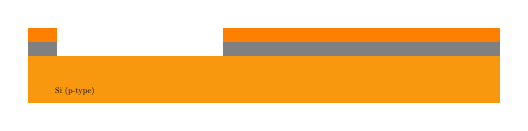
\begin{tikzpicture}[node distance = 3cm, auto, thick,scale=0.3, every node/.style={transform shape}]
		% substrate
		\fill[YellowOrange] (0,0) rectangle (20,2);
		\node at (2,0.5) {Si (p-type)};
		% oxide
		\fill[gray] (0,2) rectangle (1.25,2.6);
		\fill[gray] (8.25,2) rectangle (20,2.6);
		% resist
		\fill[orange] (0,2.6) rectangle (1.25,3.2);
		\fill[orange] (8.25,2.6) rectangle (20,3.2);
	\end{tikzpicture}

	\includegraphics[scale=0.01]{down_arrow.png}

	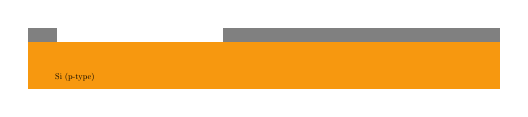
\begin{tikzpicture}[node distance = 3cm, auto, thick,scale=0.3, every node/.style={transform shape}]
		% substrate
		\fill[YellowOrange] (0,0) rectangle (20,2);
		\node at (2,0.5) {Si (p-type)};
		% oxide
		\fill[gray] (0,2) rectangle (1.25,2.6);
		\fill[gray] (8.25,2) rectangle (20,2.6);
	\end{tikzpicture}
\end{center}

\subsubsection{Predeposition}
\begin{center}
	\begin{tikzpicture}[node distance = 3cm, auto, thick,scale=0.3, every node/.style={transform shape}]
		% substrate
		\fill[YellowOrange] (0,0) rectangle (20,2);
		\node at (2,0.5) {Si (p-type)};
		% oxide
		\fill[gray] (0,2) rectangle (1.25,2.6);
		\fill[gray] (8.25,2) rectangle (20,2.6);

		\newcounter{ct}
		\forloop{ct}{0}{\value{ct} < 21}
		{
			\draw [->] (\value{ct},4) -- (\value{ct},3);
			\node at (\value{ct},4.2) {P$^{31}$};
		}
	\end{tikzpicture}

	\includegraphics[scale=0.01]{down_arrow.png}

	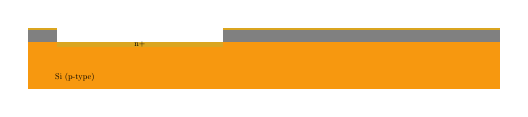
\begin{tikzpicture}[node distance = 3cm, auto, thick,scale=0.3, every node/.style={transform shape}]
		% substrate
		\fill[YellowOrange] (0,0) rectangle (20,2);
		\node at (2,0.5) {Si (p-type)};
		% phosphorus
		\fill[Goldenrod] (1.25,1.8) rectangle (8.25,2);
		\node at (4.75,1.9) {n+};
		% oxide
		\fill[gray] (0,2) rectangle (1.25,2.6);
		\fill[gray] (8.25,2) rectangle (20,2.6);

		\fill[Goldenrod] (0,2.5) rectangle (1.25,2.6);
		\fill[Goldenrod] (8.25,2.5) rectangle (20,2.6);
	\end{tikzpicture}
\end{center}

The n-well is implanted with a Phosphorus ($P^{31}$) dose of $2.5\times10^{12}cm^{-2}$ at an energy of 100 KeV.
The n-well is then annealed.

\subsubsection{Sacrificial oxide}
\begin{center}
	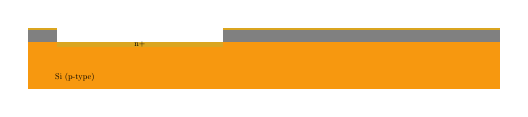
\begin{tikzpicture}[node distance = 3cm, auto, thick,scale=0.3, every node/.style={transform shape}]
		% substrate
		\fill[YellowOrange] (0,0) rectangle (20,2);
		\node at (2,0.5) {Si (p-type)};
		% phosphorus
		\fill[Goldenrod] (1.25,1.8) rectangle (8.25,2);
		\node at (4.75,1.9) {n+};
		% oxide
		\fill[gray] (0,2) rectangle (1.25,2.6);
		\fill[gray] (8.25,2) rectangle (20,2.6);

		\fill[Goldenrod] (0,2.5) rectangle (1.25,2.6);
		\fill[Goldenrod] (8.25,2.5) rectangle (20,2.6);
	\end{tikzpicture}

	\includegraphics[scale=0.01]{down_arrow.png}

	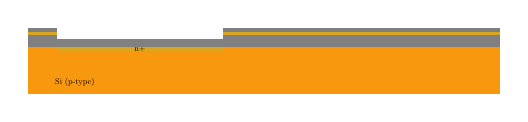
\begin{tikzpicture}[node distance = 3cm, auto, thick,scale=0.3, every node/.style={transform shape}]
		% substrate
		\fill[YellowOrange] (0,0) rectangle (20,2);
		\node at (2,0.5) {Si (p-type)};
		% phosphorus
		\fill[Goldenrod] (1.25,1.8) rectangle (8.25,2.0);
		\node at (4.75,1.9) {n+};
		% oxide
		\fill[gray] (0,2) rectangle (1.25,2.8);
		\fill[gray] (1.25,2) rectangle (8.25,2.3);
		\fill[gray] (8.25,2) rectangle (20,2.8);
		
		\fill[Goldenrod] (0,2.5) rectangle (1.25,2.6);
		\fill[Goldenrod] (8.25,2.5) rectangle (20,2.6);
	\end{tikzpicture}
\end{center}

The wafer is being oxidized for 32 minutes at 1000\degree C in order to achieve a cover silicon layer of 250nm thickness ($\approx$2500\normalfont\AA).

\subsubsection{Infusion}
In order to drive the carrier atoms deeper into the crystalline structure the wafer needs to be driven in after predeposition.
\begin{center}
	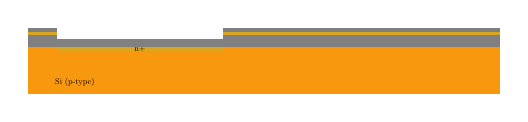
\begin{tikzpicture}[node distance = 3cm, auto, thick,scale=0.3, every node/.style={transform shape}]
		% substrate
		\fill[YellowOrange] (0,0) rectangle (20,2);
		\node at (2,0.5) {Si (p-type)};
		% phosphorus
		\fill[Goldenrod] (1.25,1.8) rectangle (8.25,2.0);
		\node at (4.75,1.9) {n+};
		% oxide
		\fill[gray] (0,2) rectangle (1.25,2.8);
		\fill[gray] (1.25,2) rectangle (8.25,2.3);
		\fill[gray] (8.25,2) rectangle (20,2.8);
		
		\fill[Goldenrod] (0,2.5) rectangle (1.25,2.6);
		\fill[Goldenrod] (8.25,2.5) rectangle (20,2.6);
	\end{tikzpicture}

	\includegraphics[scale=0.01]{down_arrow.png}

	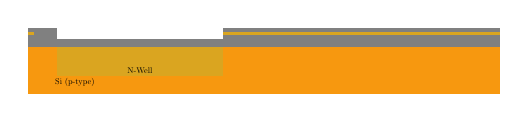
\begin{tikzpicture}[node distance = 3cm, auto, thick,scale=0.3, every node/.style={transform shape}]
		% substrate
		\fill[YellowOrange] (0,0) rectangle (20,2);
		\node at (2,0.5) {Si (p-type)};
		% n-well
		\fill[Goldenrod] (1.25,0.75) rectangle (8.25,2);
		\node at (4.75,1) {N-Well};
		% oxide
		\fill[gray] (0,2) rectangle (1.25,2.8);
		\fill[gray] (1.25,2) rectangle (8.25,2.3);
		\fill[gray] (8.25,2) rectangle (20,2.8);
		
		\fill[Goldenrod] (0,2.5) rectangle (0.25,2.6);
		\fill[Goldenrod] (8.25,2.5) rectangle (20,2.6);
	\end{tikzpicture}
\end{center}
In this step the wafer is  driven-in for 960 minutes at 1150\degree C in an inert ambient.

\subsubsection{Oxide removal}
We want an oxide free wafer with the n-well accessible for the further process steps.
\begin{center}
	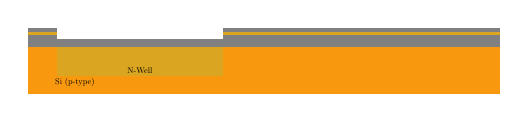
\begin{tikzpicture}[node distance = 3cm, auto, thick,scale=0.3, every node/.style={transform shape}]
		% substrate
		\fill[YellowOrange] (0,0) rectangle (20,2);
		\node at (2,0.5) {Si (p-type)};
		% n-well
		\fill[Goldenrod] (1.25,0.75) rectangle (8.25,2);
		\node at (4.75,1) {N-Well};
		% oxide
		\fill[gray] (0,2) rectangle (1.25,2.8);
		\fill[gray] (1.25,2) rectangle (8.25,2.3);
		\fill[gray] (8.25,2) rectangle (20,2.8);
		
		\fill[Goldenrod] (0,2.5) rectangle (1.25,2.6);
		\fill[Goldenrod] (8.25,2.5) rectangle (20,2.6);
	\end{tikzpicture}
	
	\includegraphics[scale=0.01]{down_arrow.png}

	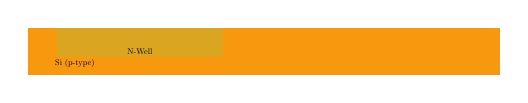
\begin{tikzpicture}[node distance = 3cm, auto, thick,scale=0.3, every node/.style={transform shape}]
		% substrate
		\fill[YellowOrange] (0,0) rectangle (20,2);
		\node at (2,0.5) {Si (p-type)};
		% n-well
		\fill[Goldenrod] (1.25,0.75) rectangle (8.25,2);
		\node at (4.75,1) {N-Well};
	\end{tikzpicture}
\end{center}

We use hydrofluoric acid, because it doesn't etch silicon at all but is very aggressive towards $SiO_2$

For hydrofluoric acid in combination with $SiO_2$ the following reaction formula can be used
\begin{equation}
4 H F_{(aq]} + SiO_{2(s]} \rightarrow SiF_{4(g]} \uparrow + 2 H_{2} O_{(l]}
\end{equation}
while with non oxidized silicon there is no reaction.
\newpage
\section{n+ Implant}\label{nimplant}
For the bulk of the PMOS transistors and for the source and drain of the NMOS transistors highly doped  n+ areas are required.
In this step we're going to build these.

\begin{figure}[H]
	\centering
	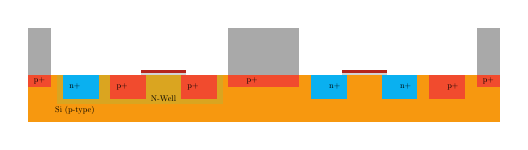
\begin{tikzpicture}[node distance = 3cm, auto, thick,scale=\CrossAndTopSectionBig, every node/.style={transform shape}]
		% substrate
\fill[YellowOrange] (0,0) rectangle (20,2);
\node at (2,0.5) {Si (p-type)};
% n-well
\fill[Goldenrod] (1.25,0.75) rectangle (8.25,2);
\node at (5.75,1) {N-Well};
% body
\fill[ProcessBlue] (1.5,1) rectangle (3,2);
\node at (2,1.5) {n+};
% source
\fill[RedOrange] (3.5,1) rectangle (5,2);
\node at (4,1.5) {p+};
% drain
\fill[RedOrange] (6.5,1) rectangle (8,2);
\node at (7,1.5) {p+};
%% gate:
% gate oxide
\fill[LightGray] (4.8,2) rectangle (6.7,2.1);
% gate poly
\fill[BrickRed] (4.8,2.1) rectangle (6.7,2.2);

%field oxides:
\fill[DarkGray] (0,2) rectangle (1,4);
\fill[DarkGray] (8.5,2) rectangle (11.5,4);
\fill[DarkGray] (19,2) rectangle (20,4);

\fill[RedOrange] (0,1.5) rectangle (1,2);
\fill[RedOrange] (8.5,1.5) rectangle (11.5,2);
\fill[RedOrange] (19,1.5) rectangle (20,2);

\node at (0.5,1.75) {p+};
\node at (9.5,1.75) {p+};
\node at (19.5,1.75) {p+};

%%% nmos:
% body
\fill[RedOrange] (17,1) rectangle (18.5,2);
\node at (18,1.5) {p+};
% source
\fill[ProcessBlue] (15,1) rectangle (16.5,2);
\node at (16,1.5) {n+};
% drain
\fill[ProcessBlue] (12,1) rectangle (13.5,2);
\node at (13,1.5) {n+};

%% gate:
% gate oxide
\fill[LightGray] (13.3,2) rectangle (15.2,2.1);
% gate poly
\fill[BrickRed] (13.3,2.1) rectangle (15.2,2.2);
	\end{tikzpicture}
	\begin{tikzpicture}[node distance = 3cm, auto, thick,scale=\CrossAndTopSectionBig, every node/.style={transform shape}]
		\fill[isolationoxide] (0,0) rectangle (20,10);

% n-well
\fill[nwell] (1,1.25) rectangle (8.5,7.5);

% p-well
\fill[pwell] (11.5,1.25) rectangle (19,7.5);

% gate metal
\fill[gatemetal] (5,0) rectangle (6.5,9);
\fill[gatemetal] (13.5,0) rectangle (15,9);
\fill[gatemetal] (5,8) rectangle (15,10);

% n+
\fill[nimplant] (1.5,2) rectangle (3,6.5);
\fill[nimplant] (12,2) rectangle (13.5,6.5);
\fill[nimplant] (15,2) rectangle (16.5,6.5);

	\end{tikzpicture}
	\caption{N+ implant geometry target}
\end{figure}

The tricky thing here is to have a reasonable implant depth but not too deep because the deeper the junction, the higher the junction capacity which in turn limits the switching performance of the CMOS circuitry.

\begin{figure}[H]
	\centering
	\begin{tikzpicture}[node distance =1cm, auto, thick,scale=\VLSILayout, every node/.style={transform shape}]
		\input{tikz_process_steps/pimplant.layout.tex}
% gate metal
\fill[gatemetal,opacity=\OpacityLayout] (4.8,1.75) rectangle (6.7,8);
\fill[gatemetal,opacity=\OpacityLayout] (13.3,1.75) rectangle (15.2,8);
\fill[gatemetal,opacity=\OpacityLayout] (4.8,8) rectangle (15.2,10);


% n+
\fill[nimplant,opacity=\OpacityLayout] (1.5,2) rectangle (3,6.5);
\fill[nimplant,opacity=\OpacityLayout] (12,2) rectangle (13.5,6.5);
\fill[nimplant,opacity=\OpacityLayout] (15,2) rectangle (16.5,6.5);

	\end{tikzpicture}
	\caption{N+ layout}
	\label{nimplant_layout}
\end{figure}

An example layout of p-implants can be seen in \autoref{nimplant_layout}, the mask is being extracted from the layer "n\_plus\_select".

Also important to notice is that this example layout is just for demonstration purposes only, please have a look at the standard cell documentation for the actual layouts. 

\newpage

\subsection{Mask dioxide layer}

In order to selectively inject charge carrying atoms into the crystalline structure a protective dioxide ($SiO_2$) layer needs to be grown on top of a p-type substrate.

\begin{figure}[H]
	\centering
	\begin{tikzpicture}[node distance = 3cm, auto, thick,scale=\CrossSectionOnly, every node/.style={transform shape}]
		\input{tikz_process_steps/nimplant.oxide_growth.a.tex}
	\end{tikzpicture}
	\drawStepArrow{}
	\begin{tikzpicture}[node distance = 3cm, auto, thick,scale=\CrossSectionOnly, every node/.style={transform shape}]
		\input{tikz_process_steps/nimplant.oxide_growth.b.tex}
	\end{tikzpicture}
	\caption{Oxide layer}
\end{figure}

With an energy of 100keV for the implantation performed in \autoref{pwell_implant_step}, the projected range of the dopants within the oxide will be 310nm (380nm tops) \footnote{\url{http://cleanroom.byu.edu/rangestraggle}}.
This means being on the safe side and having 500nm as the thickness is a good approach.
In order to grow the 500nm thick oxide layer, the wafer is being oxidized for around 56 minutes at 1050\degree C using wet oxidation which results in a dioxide layer of around 500nm in thickness\footnote{\url{http://cleanroom.byu.edu/OxideTimeCalc}}.

\subsection{Pattering}
\begin{figure}[H]
	\centering
	\begin{tikzpicture}[node distance = 3cm, auto, thick,scale=\CrossAndTopSection, every node/.style={transform shape}]
		\input{tikz_process_steps/pwell.a.tex}
\fill[gateoxide] (4.8,2) rectangle (6.7,2.3);
\fill[gateoxide] (13.3,2) rectangle (15.2,2.3);
\fill[gatemetal] (4.8,2.3) rectangle (6.7,2.6);
\fill[gatemetal] (13.3,2.3) rectangle (15.2,2.6);

	\end{tikzpicture}
	\begin{tikzpicture}[node distance = 3cm, auto, thick,scale=\CrossAndTopSection, every node/.style={transform shape}]
		\input{tikz_process_steps/nimplant.patterning.at.tex}
	\end{tikzpicture}
	\drawStepArrow{}
	\begin{tikzpicture}[node distance = 3cm, auto, thick,scale=\CrossAndTopSection, every node/.style={transform shape}]
		% resist
\fill[resist] (0,2.0) rectangle (1.25,6.0);
\fill[resist] (3,2.0) rectangle (11.75,6.0);
\fill[resist] (17,2.0) rectangle (20,6.0);

\input{tikz_process_steps/nimplant.oxide_growth.b.tex}

	\end{tikzpicture}
	\begin{tikzpicture}[node distance = 3cm, auto, thick,scale=\CrossAndTopSection, every node/.style={transform shape}]
		\fill[resist] (0,0) rectangle (20,12);

% n+
\fill[isolationoxide] (1.5,2) rectangle (3,6.5);
\fill[isolationoxide] (12,2) rectangle (13.5,6.5);
\fill[isolationoxide] (15,2) rectangle (16.5,6.5);
	\end{tikzpicture}
	\caption{N+ region resist mask}
\end{figure}

\subsection{Etching}
\begin{figure}[H]
	\centering
	\begin{tikzpicture}[node distance = 3cm, auto, thick,scale=\CrossAndTopSection, every node/.style={transform shape}]
		\input{tikz_process_steps/well.a.tex}
% oxide
\fill[isolationoxide] (0,2) rectangle (20,3);
% resist
\fill[resist] (0,3) rectangle (1.5,3.6);
\fill[resist] (3,3) rectangle (12,3.6);
\fill[resist] (13.5,3) rectangle (15,3.6);
\fill[resist] (16.5,3) rectangle (20,3.6);
	\end{tikzpicture}
	
\begin{tikzpicture}[node distance = 3cm, auto, thick,scale=\CrossAndTopSection, every node/.style={transform shape}]
		\fill[orange] (0,0) rectangle (20,12);

% n+
\fill[gray] (1.5,2) rectangle (3,6.5);
\fill[gray] (12,2) rectangle (16.5,6.5);

	\end{tikzpicture}
	\drawStepArrow{}
	\begin{tikzpicture}[node distance = 3cm, auto, thick,scale=\CrossAndTopSection, every node/.style={transform shape}]
		\input{tikz_process_steps/well.a.tex}
% gate oxide
\fill[LightGray] (4.8,2) rectangle (6.7,2.3);
\fill[LightGray] (13.3,2) rectangle (15.2,2.3);
% gate poly
\fill[BrickRed] (4.8,2.3) rectangle (6.7,2.6);
\fill[BrickRed] (13.3,2.3) rectangle (15.2,2.6);
% oxide
\fill[gray] (0,2) rectangle (1.5,3);
\fill[gray] (3,2) rectangle (4.8,3);
\fill[gray] (4.8,2.6) rectangle (6.7,3);
\fill[gray] (6.7,2) rectangle (12,3);
\fill[gray] (16.5,2) rectangle (20,3);

% resist
\fill[orange] (0,3) rectangle (1.5,3.6);
\fill[orange] (3,3) rectangle (12,3.6);
\fill[orange] (16.5,3) rectangle (20,3.6);;
	\end{tikzpicture}
	\begin{tikzpicture}[node distance = 3cm, auto, thick,scale=\CrossAndTopSection, every node/.style={transform shape}]
		\fill[resist] (0,0) rectangle (20,12);

% n+
\fill[nwell] (1.5,2) rectangle (3,6.5);
\fill[substrate] (12,2) rectangle (13.5,6.5);
\fill[substrate] (15,2) rectangle (16.5,6.5);
	\end{tikzpicture}
	\caption{N+ region opened}
\end{figure}

\subsection{Cleaning}
\begin{figure}[H]
	\centering
	\begin{tikzpicture}[node distance = 3cm, auto, thick,scale=\CrossSectionOnly, every node/.style={transform shape}]
		\input{tikz_process_steps/nimplant.4.a.tex}
	\end{tikzpicture}
	\drawStepArrow{}
	\begin{tikzpicture}[node distance = 3cm, auto, thick,scale=\CrossSectionOnly, every node/.style={transform shape}]
		\input{tikz_process_steps/well.a.tex}
% oxide
\fill[gray] (0,2) rectangle (3.5,3);
\fill[gray] (5,2) rectangle (6.5,3);
\fill[gray] (8,2) rectangle (17,3);
\fill[gray] (18.5,2) rectangle (20,3);
	\end{tikzpicture}
	\caption{Resist removal}
\end{figure}

\subsection{Implantation/Doping}\label{nimplant_implant_step}

We now need to bring in the carriers in order to build the n-junctions.

\begin{figure}[H]
	\centering
	\begin{tikzpicture}[node distance = 3cm, auto, thick,scale=\CrossSectionOnly, every node/.style={transform shape}]
		\input{tikz_process_steps/well.a.tex}
% oxide
\fill[isolationoxide] (0,2) rectangle (1.5,3);
\fill[isolationoxide] (3,2) rectangle (12,3);
\fill[isolationoxide] (13.5,2) rectangle (15,3);
\fill[isolationoxide] (16.5,2) rectangle (20,3);

\forloop{ct}{0}{\value{ct} < 21}
{
	\draw [->] (\value{ct},4) -- (\value{ct},3);
	\node at (\value{ct},4.2) {P$^{31}$};
}
	\end{tikzpicture}
	\drawStepArrow{}
	\begin{tikzpicture}[node distance = 3cm, auto, thick,scale=\CrossSectionOnly, every node/.style={transform shape}]
		\input{tikz_process_steps/nwell.a.tex}
% p-well
\fill[pwell] (11.5,0.75) rectangle (19,2);
\node at (14.25,1) {P-Well};
% oxide
\fill[isolationoxide] (0,2) rectangle (1.5,3);
\fill[isolationoxide] (3,2) rectangle (12,3);
\fill[isolationoxide] (13.5,2) rectangle (15,3);
\fill[isolationoxide] (16.5,2) rectangle (20,3);

\fill[nimplant] (1.5,1) rectangle (3,2);
\node at (2,1.5) {n+};
\fill[nimplant] (15,1) rectangle (16.5,2);
\node at (16,1.5) {n+};
\fill[nimplant] (12,1) rectangle (13.5,2);
\node at (13,1.5) {n+};
	\end{tikzpicture}
	\caption{N+ injection process}
\end{figure}

\textbf{Possible approaches}:
\begin{itemize}
	\item \textbf{"CF-3000 Implanter (IMP-3000)" from HKUST} \\
	At HKUST we have an implanter which gives us better control over the initial surface concentration. \\
	These steps are needed to arrive with the desired geometry:
	\begin{enumerate}
		\item Preparing by default cleaning
		\item The N-well is implanted with a Phosphorus ($P^{31}$) dose of $2.5\times10^{12}cm^{-2}$ at an energy of 100 keV.
		\item The N-well is annealed for 30 minutes at 1050\degreesC in $N_2$ environment (DIF-A1)\\
		After that the P-well will be around 2\um deep and the N-Well around 1\um deep
	\end{enumerate}
	\item \textbf{Constant source diffusion} \\
	We can add a layer of Phosphorus solution and diffusing in order to have an initial concentration in order to reach the desired concentration later by main diffusion.
\end{itemize}

\subsection{Oxide removal}
\begin{figure}[H]
	\centering
	\begin{tikzpicture}[node distance = 3cm, auto, thick,scale=\CrossSectionOnly, every node/.style={transform shape}]
		\input{tikz_process_steps/well.a.tex}
% gate oxide
\fill[LightGray] (4.8,2) rectangle (6.7,2.3);
\fill[LightGray] (13.3,2) rectangle (15.2,2.3);
% gate poly
\fill[BrickRed] (4.8,2.3) rectangle (6.7,2.6);
\fill[BrickRed] (13.3,2.3) rectangle (15.2,2.6);
% oxide
\fill[gray] (0,2) rectangle (1.5,3);
\fill[gray] (3,2) rectangle (4.8,3);
\fill[gray] (4.8,2.6) rectangle (6.7,3);
\fill[gray] (6.7,2) rectangle (12,3);
\fill[gray] (16.5,2) rectangle (20,3);

\fill[ProcessBlue] (1.5,1) rectangle (3,2);
\node at (2,1.5) {n+};
\fill[ProcessBlue] (15,1) rectangle (16.5,2);
\node at (16,1.5) {n+};
\fill[ProcessBlue] (12,1) rectangle (13.5,2);
\node at (13,1.5) {n+};
	\end{tikzpicture}
	\drawStepArrow{}
	\begin{tikzpicture}[node distance = 3cm, auto, thick,scale=\CrossSectionOnly, every node/.style={transform shape}]
		\input{tikz_process_steps/well.a.tex}
\fill[nimplant] (1.5,1) rectangle (3,2);
\node at (2,1.5) {n+};
\fill[nimplant] (15,1) rectangle (16.5,2);
\node at (16,1.5) {n+};
\fill[nimplant] (12,1) rectangle (13.5,2);
\node at (13,1.5) {n+};
	\end{tikzpicture}
	\caption{Oxide removal}
\end{figure}

\newpage
\section{p+ Implant}\label{pimplant}
For the bulk of the NMOS transistors and for the source and drain of the PMOS transistors highly doped  p+ areas are required.
In this step we're going to build these.

\begin{figure}[H]
	\centering
	\begin{tikzpicture}[node distance = 3cm, auto, thick,scale=\CrossAndTopSectionBig, every node/.style={transform shape}]
		% substrate
\fill[YellowOrange] (0,0) rectangle (20,2);
\node at (2,0.5) {Si (p-type)};
% n-well
\fill[Goldenrod] (1.25,0.75) rectangle (8.25,2);
\node at (5.75,1) {N-Well};
% body
\fill[ProcessBlue] (1.5,1) rectangle (3,2);
\node at (2,1.5) {n+};
% source
\fill[RedOrange] (3.5,1) rectangle (5,2);
\node at (4,1.5) {p+};
% drain
\fill[RedOrange] (6.5,1) rectangle (8,2);
\node at (7,1.5) {p+};
%% gate:
% gate oxide
\fill[LightGray] (4.8,2) rectangle (6.7,2.1);
% gate poly
\fill[BrickRed] (4.8,2.1) rectangle (6.7,2.2);

%field oxides:
\fill[DarkGray] (0,2) rectangle (1,4);
\fill[DarkGray] (8.5,2) rectangle (11.5,4);
\fill[DarkGray] (19,2) rectangle (20,4);

\fill[RedOrange] (0,1.5) rectangle (1,2);
\fill[RedOrange] (8.5,1.5) rectangle (11.5,2);
\fill[RedOrange] (19,1.5) rectangle (20,2);

\node at (0.5,1.75) {p+};
\node at (9.5,1.75) {p+};
\node at (19.5,1.75) {p+};

%%% nmos:
% body
\fill[RedOrange] (17,1) rectangle (18.5,2);
\node at (18,1.5) {p+};
% source
\fill[ProcessBlue] (15,1) rectangle (16.5,2);
\node at (16,1.5) {n+};
% drain
\fill[ProcessBlue] (12,1) rectangle (13.5,2);
\node at (13,1.5) {n+};

%% gate:
% gate oxide
\fill[LightGray] (13.3,2) rectangle (15.2,2.1);
% gate poly
\fill[BrickRed] (13.3,2.1) rectangle (15.2,2.2);
\fill[pimplant] (3.5,1) rectangle (5,2);
\node at (4,1.5) {p+};
\fill[pimplant] (6.5,1) rectangle (8,2);
\node at (7,1.5) {p+};
\fill[pimplant] (17,1) rectangle (18.5,2);
\node at (18,1.5) {p+};
	\end{tikzpicture}
	
\begin{tikzpicture}[node distance = 3cm, auto, thick,scale=\CrossAndTopSectionBig, every node/.style={transform shape}]
		\fill[YellowOrange] (0,0) rectangle (20,10);

% n-well
\fill[Goldenrod] (1,1.25) rectangle (8.5,7.5);

% p+
\fill[RedOrange] (3.5,2) rectangle (5,6.5);
\fill[RedOrange] (6.5,2) rectangle (8,6.5);
\fill[RedOrange] (17,2) rectangle (18.5,6.5);

% n+
\fill[ProcessBlue] (1.5,2) rectangle (3,6.5);
\fill[ProcessBlue] (12,2) rectangle (13.5,6.5);
\fill[ProcessBlue] (15,2) rectangle (16.5,6.5);

% trench area
\fill[DarkGray] (0,0) rectangle (1,12);
\fill[DarkGray] (8.5,0) rectangle (11.5,12);
\fill[DarkGray] (19,0) rectangle (20,12);
\fill[DarkGray] (0,0) rectangle (20,1.25);
\fill[DarkGray] (0,7.5) rectangle (20,12);

% poly
\fill[BrickRed] (4.8,1.75) rectangle (6.7,9);
\fill[BrickRed] (13.3,1.75) rectangle (15.2,9);
\fill[BrickRed] (4.8,8) rectangle (15.2,9);
	\end{tikzpicture}
	\caption{P+ implant geometry target}
\end{figure}

The tricky thing here is to have a reasonable implant depth but not too deep because the deeper the junction, the higher the junction capacity which in turn limits the switching performance of the CMOS circuitry.

\begin{figure}[H]
	\centering
	\begin{tikzpicture}[node distance =1cm, auto, thick,scale=\VLSILayout, every node/.style={transform shape}]
		\input{tikz_process_steps/gate.layout.tex}

% n+
\fill[nimplant,opacity=\OpacityLayout] (1.5,2) rectangle (3,6.5);
\fill[nimplant,opacity=\OpacityLayout] (12,2) rectangle (13.5,6.5);
\fill[nimplant,opacity=\OpacityLayout] (15,2) rectangle (16.5,6.5);


% p+
\fill[pimplant,opacity=\OpacityLayout] (3.5,2) rectangle (5,6.5);
\fill[pimplant,opacity=\OpacityLayout] (6.5,2) rectangle (8,6.5);
\fill[pimplant,opacity=\OpacityLayout] (17,2) rectangle (18.5,6.5);
	\end{tikzpicture}
	\caption{P+ layout}
	\label{pimplant_layout}
\end{figure}

An example layout of p-implants can be seen in \autoref{pimplant_layout}, the mask is being extracted from the layer "p\_plus\_select"

Also important to notice is that this example layout is just for demonstration purposes only, please have a look at the standard cell documentation for the actual layouts. 

\newpage

\subsection{Mask dioxide layer}
\begin{figure}[H]
	\centering
	\begin{tikzpicture}[node distance = 3cm, auto, thick,scale=\CrossSectionOnly, every node/.style={transform shape}]
		\input{tikz_process_steps/pimplant.oxide_growth.a.tex}
	\end{tikzpicture}
	\drawStepArrow{}
	\begin{tikzpicture}[node distance = 3cm, auto, thick,scale=\CrossSectionOnly, every node/.style={transform shape}]
		% oxide
\fill[isolationoxide] (0,2.0) rectangle (20,4.0);

\fill[isolationoxide] (0,4.0) rectangle (0.5,4.75);
\fill[isolationoxide] (9.00,4.0) rectangle (11.0,4.75);
\fill[isolationoxide] (19.5,4.0) rectangle (20,4.75);

\filldraw[line width=0, isolationoxide] (0.5,4.75) -- (0.5,4.0) -- (1.25,4.0);
\filldraw[line width=0, isolationoxide] (8.5,4.0) -- (9.00,4.0) -- (9.00,4.75);

\filldraw[line width=0, isolationoxide] (11.0,4.75) -- (11.0,4.0) -- (11.75,4.0);
\filldraw[line width=0, isolationoxide] (18.75,4.0) -- (19.5,4.0) -- (19.5,4.75);

% substrate
\fill[YellowOrange] (0,0) rectangle (20,2);
\node at (2,0.5) {Si (p-type)};
% n-well
\fill[Goldenrod] (1.25,0.75) rectangle (8.25,2);
\node at (5.75,1) {N-Well};
% body
\fill[ProcessBlue] (1.5,1) rectangle (3,2);
\node at (2,1.5) {n+};
% source
\fill[RedOrange] (3.5,1) rectangle (5,2);
\node at (4,1.5) {p+};
% drain
\fill[RedOrange] (6.5,1) rectangle (8,2);
\node at (7,1.5) {p+};
%% gate:
% gate oxide
\fill[LightGray] (4.8,2) rectangle (6.7,2.1);
% gate poly
\fill[BrickRed] (4.8,2.1) rectangle (6.7,2.2);

%field oxides:
\fill[DarkGray] (0,2) rectangle (1,4);
\fill[DarkGray] (8.5,2) rectangle (11.5,4);
\fill[DarkGray] (19,2) rectangle (20,4);

\fill[RedOrange] (0,1.5) rectangle (1,2);
\fill[RedOrange] (8.5,1.5) rectangle (11.5,2);
\fill[RedOrange] (19,1.5) rectangle (20,2);

\node at (0.5,1.75) {p+};
\node at (9.5,1.75) {p+};
\node at (19.5,1.75) {p+};

%%% nmos:
% body
\fill[RedOrange] (17,1) rectangle (18.5,2);
\node at (18,1.5) {p+};
% source
\fill[ProcessBlue] (15,1) rectangle (16.5,2);
\node at (16,1.5) {n+};
% drain
\fill[ProcessBlue] (12,1) rectangle (13.5,2);
\node at (13,1.5) {n+};

%% gate:
% gate oxide
\fill[LightGray] (13.3,2) rectangle (15.2,2.1);
% gate poly
\fill[BrickRed] (13.3,2.1) rectangle (15.2,2.2);
	\end{tikzpicture}
	\caption{Oxide layer}
\end{figure}

\subsection{Pattering}
\begin{figure}[H]
	\centering
	\begin{tikzpicture}[node distance = 3cm, auto, thick,scale=\CrossAndTopSection, every node/.style={transform shape}]
		% substrate
\fill[YellowOrange] (0,0) rectangle (20,2);
\node at (2,0.5) {Si (p-type)};
% n-well
\fill[Goldenrod] (1.25,0.75) rectangle (8.25,2);
\node at (5.75,1) {N-Well};
% body
\fill[ProcessBlue] (1.5,1) rectangle (3,2);
\node at (2,1.5) {n+};
% source
\fill[RedOrange] (3.5,1) rectangle (5,2);
\node at (4,1.5) {p+};
% drain
\fill[RedOrange] (6.5,1) rectangle (8,2);
\node at (7,1.5) {p+};
%% gate:
% gate oxide
\fill[LightGray] (4.8,2) rectangle (6.7,2.1);
% gate poly
\fill[BrickRed] (4.8,2.1) rectangle (6.7,2.2);

%field oxides:
\fill[DarkGray] (0,2) rectangle (1,4);
\fill[DarkGray] (8.5,2) rectangle (11.5,4);
\fill[DarkGray] (19,2) rectangle (20,4);

\fill[RedOrange] (0,1.5) rectangle (1,2);
\fill[RedOrange] (8.5,1.5) rectangle (11.5,2);
\fill[RedOrange] (19,1.5) rectangle (20,2);

\node at (0.5,1.75) {p+};
\node at (9.5,1.75) {p+};
\node at (19.5,1.75) {p+};

%%% nmos:
% body
\fill[RedOrange] (17,1) rectangle (18.5,2);
\node at (18,1.5) {p+};
% source
\fill[ProcessBlue] (15,1) rectangle (16.5,2);
\node at (16,1.5) {n+};
% drain
\fill[ProcessBlue] (12,1) rectangle (13.5,2);
\node at (13,1.5) {n+};

%% gate:
% gate oxide
\fill[LightGray] (13.3,2) rectangle (15.2,2.1);
% gate poly
\fill[BrickRed] (13.3,2.1) rectangle (15.2,2.2);

	\end{tikzpicture}
	\begin{tikzpicture}[node distance = 3cm, auto, thick,scale=\CrossAndTopSection, every node/.style={transform shape}]
		\input{tikz_process_steps/pimplant.patterning.at.tex}
	\end{tikzpicture}
	\drawStepArrow{}
	\begin{tikzpicture}[node distance = 3cm, auto, thick,scale=\CrossAndTopSection, every node/.style={transform shape}]
		% resist
\fill[resist] (0,2.0) rectangle (3.75,5.0);
\fill[resist] (8.75,2.0) rectangle (16.75,5.0);
\fill[resist] (19.25,2.0) rectangle (20,5.0);

\input{tikz_process_steps/nimplant.a.tex}


	\end{tikzpicture}
	\begin{tikzpicture}[node distance = 3cm, auto, thick,scale=\CrossAndTopSection, every node/.style={transform shape}]
		\fill[resist] (0,0) rectangle (20,12);

% p+
\fill[isolationoxide] (3.5,2) rectangle (5,6.5);
\fill[isolationoxide] (6.5,2) rectangle (8,6.5);
\fill[isolationoxide] (17,2) rectangle (18.25,6.5);
	\end{tikzpicture}
	\caption{P+ region resist mask}
\end{figure}

\subsection{Etching}
\begin{figure}[H]
	\centering
	\begin{tikzpicture}[node distance = 3cm, auto, thick,scale=\CrossAndTopSection, every node/.style={transform shape}]
		% oxide
\fill[isolationoxide] (0,2) rectangle (20,3.5);
% resist
\fill[resist] (0,3.5) rectangle (3.5,4.1);
\fill[resist] (8,3.5) rectangle (17,4.1);
\fill[resist] (18.5,3.5) rectangle (20,4.1);

% substrate
\fill[YellowOrange] (0,0) rectangle (20,2);
\node at (2,0.5) {Si (p-type)};
% n-well
\fill[Goldenrod] (1.25,0.75) rectangle (8.25,2);
\node at (5.75,1) {N-Well};
% body
\fill[ProcessBlue] (1.5,1) rectangle (3,2);
\node at (2,1.5) {n+};
% source
\fill[RedOrange] (3.5,1) rectangle (5,2);
\node at (4,1.5) {p+};
% drain
\fill[RedOrange] (6.5,1) rectangle (8,2);
\node at (7,1.5) {p+};
%% gate:
% gate oxide
\fill[LightGray] (4.8,2) rectangle (6.7,2.1);
% gate poly
\fill[BrickRed] (4.8,2.1) rectangle (6.7,2.2);

%field oxides:
\fill[DarkGray] (0,2) rectangle (1,4);
\fill[DarkGray] (8.5,2) rectangle (11.5,4);
\fill[DarkGray] (19,2) rectangle (20,4);

\fill[RedOrange] (0,1.5) rectangle (1,2);
\fill[RedOrange] (8.5,1.5) rectangle (11.5,2);
\fill[RedOrange] (19,1.5) rectangle (20,2);

\node at (0.5,1.75) {p+};
\node at (9.5,1.75) {p+};
\node at (19.5,1.75) {p+};

%%% nmos:
% body
\fill[RedOrange] (17,1) rectangle (18.5,2);
\node at (18,1.5) {p+};
% source
\fill[ProcessBlue] (15,1) rectangle (16.5,2);
\node at (16,1.5) {n+};
% drain
\fill[ProcessBlue] (12,1) rectangle (13.5,2);
\node at (13,1.5) {n+};

%% gate:
% gate oxide
\fill[LightGray] (13.3,2) rectangle (15.2,2.1);
% gate poly
\fill[BrickRed] (13.3,2.1) rectangle (15.2,2.2);
	\end{tikzpicture}
	\begin{tikzpicture}[node distance = 3cm, auto, thick,scale=\CrossAndTopSection, every node/.style={transform shape}]
		\fill[orange] (0,0) rectangle (20,12);

% n+
\fill[gray] (3.5,2) rectangle (8,6.5);
\fill[gray] (17,2) rectangle (18.5,6.5);
	\end{tikzpicture}
	\drawStepArrow{}
	\begin{tikzpicture}[node distance = 3cm, auto, thick,scale=\CrossAndTopSection, every node/.style={transform shape}]
		% oxide
\fill[isolationoxide] (0,2) rectangle (3.0,3.5);
\fill[isolationoxide] (8.5,2) rectangle (17,3.5);
\fill[isolationoxide] (18.75,2) rectangle (20,3.5);

% resist
\fill[resist] (0,3.5) rectangle (3.0,4.1);
\fill[resist] (8.5,3.5) rectangle (17,4.1);
\fill[resist] (18.75,3.5) rectangle (20,4.1);

% substrate
\fill[YellowOrange] (0,0) rectangle (20,2);
\node at (2,0.5) {Si (p-type)};
% n-well
\fill[Goldenrod] (1.25,0.75) rectangle (8.25,2);
\node at (5.75,1) {N-Well};
% body
\fill[ProcessBlue] (1.5,1) rectangle (3,2);
\node at (2,1.5) {n+};
% source
\fill[RedOrange] (3.5,1) rectangle (5,2);
\node at (4,1.5) {p+};
% drain
\fill[RedOrange] (6.5,1) rectangle (8,2);
\node at (7,1.5) {p+};
%% gate:
% gate oxide
\fill[LightGray] (4.8,2) rectangle (6.7,2.1);
% gate poly
\fill[BrickRed] (4.8,2.1) rectangle (6.7,2.2);

%field oxides:
\fill[DarkGray] (0,2) rectangle (1,4);
\fill[DarkGray] (8.5,2) rectangle (11.5,4);
\fill[DarkGray] (19,2) rectangle (20,4);

\fill[RedOrange] (0,1.5) rectangle (1,2);
\fill[RedOrange] (8.5,1.5) rectangle (11.5,2);
\fill[RedOrange] (19,1.5) rectangle (20,2);

\node at (0.5,1.75) {p+};
\node at (9.5,1.75) {p+};
\node at (19.5,1.75) {p+};

%%% nmos:
% body
\fill[RedOrange] (17,1) rectangle (18.5,2);
\node at (18,1.5) {p+};
% source
\fill[ProcessBlue] (15,1) rectangle (16.5,2);
\node at (16,1.5) {n+};
% drain
\fill[ProcessBlue] (12,1) rectangle (13.5,2);
\node at (13,1.5) {n+};

%% gate:
% gate oxide
\fill[LightGray] (13.3,2) rectangle (15.2,2.1);
% gate poly
\fill[BrickRed] (13.3,2.1) rectangle (15.2,2.2);

	\end{tikzpicture}
	\begin{tikzpicture}[node distance = 3cm, auto, thick,scale=\CrossAndTopSection, every node/.style={transform shape}]
		\fill[orange] (0,0) rectangle (20,12);

% p+
\fill[Goldenrod] (3.5,2) rectangle (5,6.5);
\fill[Goldenrod] (6.5,2) rectangle (8,6.5);
\fill[YellowOrange] (17,2) rectangle (18.5,6.5);
	\end{tikzpicture}
	\caption{P+ region opened}
\end{figure}

\subsection{Cleaning}
\begin{figure}[H]
	\centering
	\begin{tikzpicture}[node distance = 3cm, auto, thick,scale=\CrossSectionOnly, every node/.style={transform shape}]
		% substrate
\fill[YellowOrange] (0,0) rectangle (20,2);
\node at (2,0.5) {Si (p-type)};
% n-well
\fill[Goldenrod] (1.25,0.75) rectangle (8.25,2);
\node at (5.75,1) {N-Well};
% body
\fill[ProcessBlue] (1.5,1) rectangle (3,2);
\node at (2,1.5) {n+};
% source
\fill[RedOrange] (3.5,1) rectangle (5,2);
\node at (4,1.5) {p+};
% drain
\fill[RedOrange] (6.5,1) rectangle (8,2);
\node at (7,1.5) {p+};
%% gate:
% gate oxide
\fill[LightGray] (4.8,2) rectangle (6.7,2.1);
% gate poly
\fill[BrickRed] (4.8,2.1) rectangle (6.7,2.2);

%field oxides:
\fill[DarkGray] (0,2) rectangle (1,4);
\fill[DarkGray] (8.5,2) rectangle (11.5,4);
\fill[DarkGray] (19,2) rectangle (20,4);

\fill[RedOrange] (0,1.5) rectangle (1,2);
\fill[RedOrange] (8.5,1.5) rectangle (11.5,2);
\fill[RedOrange] (19,1.5) rectangle (20,2);

\node at (0.5,1.75) {p+};
\node at (9.5,1.75) {p+};
\node at (19.5,1.75) {p+};

%%% nmos:
% body
\fill[RedOrange] (17,1) rectangle (18.5,2);
\node at (18,1.5) {p+};
% source
\fill[ProcessBlue] (15,1) rectangle (16.5,2);
\node at (16,1.5) {n+};
% drain
\fill[ProcessBlue] (12,1) rectangle (13.5,2);
\node at (13,1.5) {n+};

%% gate:
% gate oxide
\fill[LightGray] (13.3,2) rectangle (15.2,2.1);
% gate poly
\fill[BrickRed] (13.3,2.1) rectangle (15.2,2.2);

% oxide
\fill[isolationoxide] (0,2) rectangle (3.5,3);
\fill[isolationoxide] (5,2) rectangle (6.5,3);
\fill[isolationoxide] (8,2) rectangle (17,3);
\fill[isolationoxide] (18.5,2) rectangle (20,3);;

% resist
\fill[resist] (0,3) rectangle (3.5,3.6);
\fill[resist] (5,3) rectangle (6.5,3.6);
\fill[resist] (8,3) rectangle (17,3.6);
\fill[resist] (18.5,3) rectangle (20,3.6);;
	\end{tikzpicture}
	\drawStepArrow{}
	\begin{tikzpicture}[node distance = 3cm, auto, thick,scale=\CrossSectionOnly, every node/.style={transform shape}]
		% substrate
\fill[YellowOrange] (0,0) rectangle (20,2);
\node at (2,0.5) {Si (p-type)};
% n-well
\fill[Goldenrod] (1.25,0.75) rectangle (8.25,2);
\node at (5.75,1) {N-Well};
% body
\fill[ProcessBlue] (1.5,1) rectangle (3,2);
\node at (2,1.5) {n+};
% source
\fill[RedOrange] (3.5,1) rectangle (5,2);
\node at (4,1.5) {p+};
% drain
\fill[RedOrange] (6.5,1) rectangle (8,2);
\node at (7,1.5) {p+};
%% gate:
% gate oxide
\fill[LightGray] (4.8,2) rectangle (6.7,2.1);
% gate poly
\fill[BrickRed] (4.8,2.1) rectangle (6.7,2.2);

%field oxides:
\fill[DarkGray] (0,2) rectangle (1,4);
\fill[DarkGray] (8.5,2) rectangle (11.5,4);
\fill[DarkGray] (19,2) rectangle (20,4);

\fill[RedOrange] (0,1.5) rectangle (1,2);
\fill[RedOrange] (8.5,1.5) rectangle (11.5,2);
\fill[RedOrange] (19,1.5) rectangle (20,2);

\node at (0.5,1.75) {p+};
\node at (9.5,1.75) {p+};
\node at (19.5,1.75) {p+};

%%% nmos:
% body
\fill[RedOrange] (17,1) rectangle (18.5,2);
\node at (18,1.5) {p+};
% source
\fill[ProcessBlue] (15,1) rectangle (16.5,2);
\node at (16,1.5) {n+};
% drain
\fill[ProcessBlue] (12,1) rectangle (13.5,2);
\node at (13,1.5) {n+};

%% gate:
% gate oxide
\fill[LightGray] (13.3,2) rectangle (15.2,2.1);
% gate poly
\fill[BrickRed] (13.3,2.1) rectangle (15.2,2.2);

% oxide
\fill[gray] (0,2) rectangle (3.5,3);
\fill[gray] (8,2) rectangle (13.3,3);
\fill[gray] (13.3,2.6) rectangle (15.2,3);
\fill[gray] (15.2,2) rectangle (17,3);
\fill[gray] (18.5,2) rectangle (20,3);
	\end{tikzpicture}
	\caption{Resist removal}
\end{figure}

\subsection{Implantation/Doping}\label{pimplant_implant_step}
\begin{figure}[H]
	\centering
	\begin{tikzpicture}[node distance = 3cm, auto, thick,scale=\CrossSectionOnly, every node/.style={transform shape}]
		% oxide
\fill[isolationoxide] (0,2) rectangle (3.5,3.5);
\fill[isolationoxide] (8,2) rectangle (17,3.5);
\fill[isolationoxide] (18.5,2) rectangle (20,3.5);

\forloop{ct}{0}{\value{ct} < 21}
{
	\draw [->] (\value{ct},5) -- (\value{ct},4);
	\node at (\value{ct},5.2) {B$^{11}$};
}

% substrate
\fill[YellowOrange] (0,0) rectangle (20,2);
\node at (2,0.5) {Si (p-type)};
% n-well
\fill[Goldenrod] (1.25,0.75) rectangle (8.25,2);
\node at (5.75,1) {N-Well};
% body
\fill[ProcessBlue] (1.5,1) rectangle (3,2);
\node at (2,1.5) {n+};
% source
\fill[RedOrange] (3.5,1) rectangle (5,2);
\node at (4,1.5) {p+};
% drain
\fill[RedOrange] (6.5,1) rectangle (8,2);
\node at (7,1.5) {p+};
%% gate:
% gate oxide
\fill[LightGray] (4.8,2) rectangle (6.7,2.1);
% gate poly
\fill[BrickRed] (4.8,2.1) rectangle (6.7,2.2);

%field oxides:
\fill[DarkGray] (0,2) rectangle (1,4);
\fill[DarkGray] (8.5,2) rectangle (11.5,4);
\fill[DarkGray] (19,2) rectangle (20,4);

\fill[RedOrange] (0,1.5) rectangle (1,2);
\fill[RedOrange] (8.5,1.5) rectangle (11.5,2);
\fill[RedOrange] (19,1.5) rectangle (20,2);

\node at (0.5,1.75) {p+};
\node at (9.5,1.75) {p+};
\node at (19.5,1.75) {p+};

%%% nmos:
% body
\fill[RedOrange] (17,1) rectangle (18.5,2);
\node at (18,1.5) {p+};
% source
\fill[ProcessBlue] (15,1) rectangle (16.5,2);
\node at (16,1.5) {n+};
% drain
\fill[ProcessBlue] (12,1) rectangle (13.5,2);
\node at (13,1.5) {n+};

%% gate:
% gate oxide
\fill[LightGray] (13.3,2) rectangle (15.2,2.1);
% gate poly
\fill[BrickRed] (13.3,2.1) rectangle (15.2,2.2);

	\end{tikzpicture}
	\drawStepArrow{}
	\begin{tikzpicture}[node distance = 3cm, auto, thick,scale=\CrossSectionOnly, every node/.style={transform shape}]
		% substrate
\fill[YellowOrange] (0,0) rectangle (20,2);
\node at (2,0.5) {Si (p-type)};
% n-well
\fill[Goldenrod] (1.25,0.75) rectangle (8.25,2);
\node at (5.75,1) {N-Well};
% body
\fill[ProcessBlue] (1.5,1) rectangle (3,2);
\node at (2,1.5) {n+};
% source
\fill[RedOrange] (3.5,1) rectangle (5,2);
\node at (4,1.5) {p+};
% drain
\fill[RedOrange] (6.5,1) rectangle (8,2);
\node at (7,1.5) {p+};
%% gate:
% gate oxide
\fill[LightGray] (4.8,2) rectangle (6.7,2.1);
% gate poly
\fill[BrickRed] (4.8,2.1) rectangle (6.7,2.2);

%field oxides:
\fill[DarkGray] (0,2) rectangle (1,4);
\fill[DarkGray] (8.5,2) rectangle (11.5,4);
\fill[DarkGray] (19,2) rectangle (20,4);

\fill[RedOrange] (0,1.5) rectangle (1,2);
\fill[RedOrange] (8.5,1.5) rectangle (11.5,2);
\fill[RedOrange] (19,1.5) rectangle (20,2);

\node at (0.5,1.75) {p+};
\node at (9.5,1.75) {p+};
\node at (19.5,1.75) {p+};

%%% nmos:
% body
\fill[RedOrange] (17,1) rectangle (18.5,2);
\node at (18,1.5) {p+};
% source
\fill[ProcessBlue] (15,1) rectangle (16.5,2);
\node at (16,1.5) {n+};
% drain
\fill[ProcessBlue] (12,1) rectangle (13.5,2);
\node at (13,1.5) {n+};

%% gate:
% gate oxide
\fill[LightGray] (13.3,2) rectangle (15.2,2.1);
% gate poly
\fill[BrickRed] (13.3,2.1) rectangle (15.2,2.2);
% oxide
\fill[isolationoxide] (0,2) rectangle (3.5,3);
\fill[isolationoxide] (5,2) rectangle (6.5,3);
\fill[isolationoxide] (8,2) rectangle (17,3);
\fill[isolationoxide] (18.5,2) rectangle (20,3);

\fill[pimplant] (3.5,1) rectangle (5,2);
\node at (4,1.5) {p+};
\fill[pimplant] (6.5,1) rectangle (8,2);
\node at (7,1.5) {p+};
\fill[pimplant] (17,1) rectangle (18.5,2);
\node at (18,1.5) {p+};
	\end{tikzpicture}
	\caption{P+ injection process}
\end{figure}

\subsection{Oxide removal}
\begin{figure}[H]
	\centering
	\begin{tikzpicture}[node distance = 3cm, auto, thick,scale=\CrossSectionOnly, every node/.style={transform shape}]
		% oxide
\fill[isolationoxide] (0,2) rectangle (3.0,3.5);
\fill[isolationoxide] (8.5,2) rectangle (17,3.5);
\fill[isolationoxide] (18.75,2) rectangle (20,3.5);

% substrate
\fill[YellowOrange] (0,0) rectangle (20,2);
\node at (2,0.5) {Si (p-type)};
% n-well
\fill[Goldenrod] (1.25,0.75) rectangle (8.25,2);
\node at (5.75,1) {N-Well};
% body
\fill[ProcessBlue] (1.5,1) rectangle (3,2);
\node at (2,1.5) {n+};
% source
\fill[RedOrange] (3.5,1) rectangle (5,2);
\node at (4,1.5) {p+};
% drain
\fill[RedOrange] (6.5,1) rectangle (8,2);
\node at (7,1.5) {p+};
%% gate:
% gate oxide
\fill[LightGray] (4.8,2) rectangle (6.7,2.1);
% gate poly
\fill[BrickRed] (4.8,2.1) rectangle (6.7,2.2);

%field oxides:
\fill[DarkGray] (0,2) rectangle (1,4);
\fill[DarkGray] (8.5,2) rectangle (11.5,4);
\fill[DarkGray] (19,2) rectangle (20,4);

\fill[RedOrange] (0,1.5) rectangle (1,2);
\fill[RedOrange] (8.5,1.5) rectangle (11.5,2);
\fill[RedOrange] (19,1.5) rectangle (20,2);

\node at (0.5,1.75) {p+};
\node at (9.5,1.75) {p+};
\node at (19.5,1.75) {p+};

%%% nmos:
% body
\fill[RedOrange] (17,1) rectangle (18.5,2);
\node at (18,1.5) {p+};
% source
\fill[ProcessBlue] (15,1) rectangle (16.5,2);
\node at (16,1.5) {n+};
% drain
\fill[ProcessBlue] (12,1) rectangle (13.5,2);
\node at (13,1.5) {n+};

%% gate:
% gate oxide
\fill[LightGray] (13.3,2) rectangle (15.2,2.1);
% gate poly
\fill[BrickRed] (13.3,2.1) rectangle (15.2,2.2);

\fill[pimplant] (3.0,1.5) rectangle (5,2);
\fill[pimplant] (6.5,1.5) rectangle (8.5,2);
\fill[pimplant] (17,1.5) rectangle (18.75,2);
	\end{tikzpicture}
	\drawStepArrow{}
	\begin{tikzpicture}[node distance = 3cm, auto, thick,scale=\CrossSectionOnly, every node/.style={transform shape}]
		% substrate
\fill[YellowOrange] (0,0) rectangle (20,2);
\node at (2,0.5) {Si (p-type)};
% n-well
\fill[Goldenrod] (1.25,0.75) rectangle (8.25,2);
\node at (5.75,1) {N-Well};
% body
\fill[ProcessBlue] (1.5,1) rectangle (3,2);
\node at (2,1.5) {n+};
% source
\fill[RedOrange] (3.5,1) rectangle (5,2);
\node at (4,1.5) {p+};
% drain
\fill[RedOrange] (6.5,1) rectangle (8,2);
\node at (7,1.5) {p+};
%% gate:
% gate oxide
\fill[LightGray] (4.8,2) rectangle (6.7,2.1);
% gate poly
\fill[BrickRed] (4.8,2.1) rectangle (6.7,2.2);

%field oxides:
\fill[DarkGray] (0,2) rectangle (1,4);
\fill[DarkGray] (8.5,2) rectangle (11.5,4);
\fill[DarkGray] (19,2) rectangle (20,4);

\fill[RedOrange] (0,1.5) rectangle (1,2);
\fill[RedOrange] (8.5,1.5) rectangle (11.5,2);
\fill[RedOrange] (19,1.5) rectangle (20,2);

\node at (0.5,1.75) {p+};
\node at (9.5,1.75) {p+};
\node at (19.5,1.75) {p+};

%%% nmos:
% body
\fill[RedOrange] (17,1) rectangle (18.5,2);
\node at (18,1.5) {p+};
% source
\fill[ProcessBlue] (15,1) rectangle (16.5,2);
\node at (16,1.5) {n+};
% drain
\fill[ProcessBlue] (12,1) rectangle (13.5,2);
\node at (13,1.5) {n+};

%% gate:
% gate oxide
\fill[LightGray] (13.3,2) rectangle (15.2,2.1);
% gate poly
\fill[BrickRed] (13.3,2.1) rectangle (15.2,2.2);

\fill[RedOrange] (3.5,1) rectangle (5,2);
\node at (4,1.5) {p+};
\fill[RedOrange] (6.5,1) rectangle (8,2);
\node at (7,1.5) {p+};
\fill[RedOrange] (17,1) rectangle (18.5,2);
\node at (18,1.5) {p+};
	\end{tikzpicture}
	\caption{Oxide removal}
\end{figure}

\newpage
\section{Gate}\label{gate}
Now we have to build the initial gate structure which contains of the 40nm thick dielectric (in our case just silicon dioxide) and the polysilicon electrode.

\begin{figure}[H]
	\centering
	\begin{tikzpicture}[node distance = 3cm, auto, thick,scale=\CrossAndTopSectionBig, every node/.style={transform shape}]
		\input{tikz_process_steps/nwell.a.tex}
% p-well
\fill[pwell] (11.5,0.75) rectangle (19,2);
\node at (14.25,1) {P-Well};
\fill[gateoxide] (4.8,2) rectangle (6.7,2.3);
\fill[gateoxide] (13.3,2) rectangle (15.2,2.3);
\fill[gatemetal] (4.8,2.3) rectangle (6.7,2.6);
\fill[gatemetal] (13.3,2.3) rectangle (15.2,2.6);
		\node at (3,3) {Gate oxide};
		\draw[->] (3,2.8) -- (5,2.2);
		\node at (3,4) {Polysilicon};
		\draw[->] (3,3.8) -- (5,3.2);
	\end{tikzpicture}
	\begin{tikzpicture}[node distance = 3cm, auto, thick,scale=\CrossAndTopSectionBig, every node/.style={transform shape}]
		\input{tikz_process_steps/nwell.b.tex}
\fill[pwell] (11.5,1.25) rectangle (19,7.5);

% gate metal
\fill[gatemetal] (5,0) rectangle (6.5,9);
\fill[gatemetal] (13.5,0) rectangle (15,9);
\fill[gatemetal] (5,8) rectangle (15,10);
	\end{tikzpicture}
	\caption{Poly silicon gate contacts with gate oxide}
\end{figure}

The line spacing of the polysilicon electrode shape has to be at least 0.5\um because of the resolution of the stepper and also because of the etching process which has 0.5\um as the minimum line spacing.

\begin{figure}[H]
	\centering
	\begin{tikzpicture}[node distance =1cm, auto, thick,scale=\VLSILayout, every node/.style={transform shape}]
		\input{tikz_process_steps/nimplant.layout.tex}

% p+
\fill[pimplant,opacity=\OpacityLayout] (3.5,2) rectangle (5,6.5);
\fill[pimplant,opacity=\OpacityLayout] (6.5,2) rectangle (8,6.5);
\fill[pimplant,opacity=\OpacityLayout] (17,2) rectangle (18.5,6.5);
% gate metal
\fill[gatemetal,opacity=\OpacityLayout] (4.8,1.75) rectangle (6.7,8);
\fill[gatemetal,opacity=\OpacityLayout] (13.3,1.75) rectangle (15.2,8);
\fill[gatemetal,opacity=\OpacityLayout] (4.8,8) rectangle (15.2,10);

	\end{tikzpicture}
	\caption{Gate layout}
	\label{gate_layout}
\end{figure}

In \autoref{gate_layout} we can see the layout honoring the 0.5\um spacing design rule for the gate structure shape and poly-layer interconnect between NMOS and PMOS.

\newpage

\subsection{Gate oxide deposition}

Now we have to deposit the dielectric isolator between the gate electrode and the channel.
As designed in the process design document, the layer will be 40nm thick.

\begin{figure}[H]
	\centering
	\begin{tikzpicture}[node distance = 3cm, auto, thick,scale=\CrossSectionOnly, every node/.style={transform shape}]
		\def\welldepthAfox{0.75}
\def\welldepthBfox{1.25}
\def\welldepthCfox{1.5}

\newcommand{\stopper}[1]{
\filldraw[line width=0, isolationoxide] (#1,2.0) -- (#1+0.75,2.0) -- (#1+0.75,2.75);
\fill[isolationoxide] (#1+0.75,2.0) rectangle (#1+1.25,2.75);
\filldraw[line width=0, isolationoxide] (#1+1.25,2.75) -- (#1+1.25,2.0) -- (#1+2.0,2.0);
}

\newcommand{\bjtstopper}[1]{
\filldraw[line width=0, isolationoxide] (#1,2.0) -- (#1+0.25,2.0) -- (#1+0.25,2.75);
\fill[isolationoxide] (#1+0.25,2.0) rectangle (#1+0.5,2.75);
\filldraw[line width=0, isolationoxide] (#1+0.5,2.75) -- (#1+0.5,2.0) -- (#1+0.75,2.0);
}

% oxide
\fill[isolationoxide] (0,1.25) rectangle (55.0,2.0);

\fill[isolationoxide] (0,2.0) rectangle (0.75,2.75);
\filldraw[line width=0, isolationoxide] (0.75,2.75) -- (0.75,2.0) -- (1.5,2.0);

%separates n+ from p+
\stopper{2.5}
\stopper{8.0}

%separates n+ from p+
\stopper{13.5}

\stopper{16.5}
\stopper{17.0}

\stopper{20.0}

\stopper{24.5}
\stopper{25.0}

\bjtstopper{27.75}
\bjtstopper{29.0}
\bjtstopper{30.5}
\bjtstopper{31.75}

\stopper{33.5}
\stopper{33.75}

\bjtstopper{36.5}
\bjtstopper{37.75}
\bjtstopper{39.0}
\bjtstopper{40.25}

\filldraw[line width=0, isolationoxide] (41.75,2.0) -- (42.5,2.0) -- (42.5,2.75);
\fill[isolationoxide] (42.5,2.0) rectangle (55.0,2.75);

\input{tikz_process_steps/sti.a.tex}

% substrate
\fill[substrate] (0,0) rectangle (55,1.25);
\node at (2,0.5) {Silicon substrate};

% normal wells
\shade[upper left = nwell, upper right = nwell, lower right = substrate, lower left = substrate,] (1.25,\welldepthAfox) rectangle (8.25,2.0);
\shade[upper left = pwell, upper right = pwell, lower right = substrate, lower left = substrate,] (9.75,\welldepthAfox) rectangle (16.75,2.0);
\shade[upper left = nwell, upper right = nwell, lower right = substrate, lower left = substrate,] (18.25,\welldepthAfox) rectangle (25.25,2.0);
\shade[upper left = nwell, upper right = nwell, lower right = substrate, lower left = substrate,] (26.75,\welldepthAfox) rectangle (33.75,2.0);
\shade[upper left = nwell, upper right = nwell, lower right = substrate, lower left = substrate,] (35.25,\welldepthAfox) rectangle (42.25,2.0);

% p base
\shade[upper left = pbase, upper right = pbase, lower right = nwell, lower left = nwell,] (18.5,\welldepthBfox) rectangle (25.0,2.0);

% npn - pbase
\shade[upper left = pbase, upper right = pbase, lower right = nwell, lower left = nwell,] (28.25,\welldepthBfox) rectangle (32.0,2.0);

% pnp emitter and collector ring
\shade[upper left = pbase, upper right = pbase, lower right = nwell, lower left = nwell,] (35.5,\welldepthBfox) rectangle (37.0,2.0);
\shade[upper left = pbase, upper right = pbase, lower right = nwell, lower left = nwell,] (38.0,\welldepthBfox) rectangle (39.5,2.0);
\shade[upper left = pbase, upper right = pbase, lower right = nwell, lower left = nwell,] (40.5,\welldepthBfox) rectangle (42.0,2.0);

% n base for SONOS
\shade[upper left = nbase, upper right = nbase, lower right = pbase, lower left = pbase,] (18.75,\welldepthCfox) rectangle (24.75,2.0);

% n base for NPN emitter
\shade[upper left = nbase, upper right = nbase, lower right = pbase, lower left = pbase,] (29.5,\welldepthCfox) rectangle (30.75,2.0);


	\end{tikzpicture} \\
	\includegraphics[scale=0.01]{down_arrow.png} \\
	\begin{tikzpicture}[node distance = 3cm, auto, thick,scale=\CrossSectionOnly, every node/.style={transform shape}]
		\def\welldepthAfox{0.75}
\def\welldepthBfox{1.25}
\def\welldepthCfox{1.5}

\newcommand{\stopper}[1]{
\filldraw[line width=0, isolationoxide] (#1,2.0) -- (#1+0.75,2.0) -- (#1+0.75,2.75);
\fill[isolationoxide] (#1+0.75,2.0) rectangle (#1+1.25,2.75);
\filldraw[line width=0, isolationoxide] (#1+1.25,2.75) -- (#1+1.25,2.0) -- (#1+2.0,2.0);
}

\newcommand{\bjtstopper}[1]{
\filldraw[line width=0, isolationoxide] (#1,2.0) -- (#1+0.25,2.0) -- (#1+0.25,2.75);
\fill[isolationoxide] (#1+0.25,2.0) rectangle (#1+0.5,2.75);
\filldraw[line width=0, isolationoxide] (#1+0.5,2.75) -- (#1+0.5,2.0) -- (#1+0.75,2.0);
}

% oxide
\fill[isolationoxide] (0,1.25) rectangle (55.0,2.0);

\fill[isolationoxide] (0,2.0) rectangle (0.75,2.75);
\filldraw[line width=0, isolationoxide] (0.75,2.75) -- (0.75,2.0) -- (1.5,2.0);

%separates n+ from p+
\stopper{2.5}
\stopper{8.0}

%separates n+ from p+
\stopper{13.5}

\stopper{16.5}
\stopper{17.0}

\stopper{20.0}

\stopper{24.5}
\stopper{25.0}

\bjtstopper{27.75}
\bjtstopper{29.0}
\bjtstopper{30.5}
\bjtstopper{31.75}

\stopper{33.5}
\stopper{33.75}

\bjtstopper{36.5}
\bjtstopper{37.75}
\bjtstopper{39.0}
\bjtstopper{40.25}

\filldraw[line width=0, isolationoxide] (41.75,2.0) -- (42.5,2.0) -- (42.5,2.75);
\fill[isolationoxide] (42.5,2.0) rectangle (55.0,2.75);

\input{tikz_process_steps/sti.a.tex}

% substrate
\fill[substrate] (0,0) rectangle (55,1.25);
\node at (2,0.5) {Silicon substrate};

% normal wells
\shade[upper left = nwell, upper right = nwell, lower right = substrate, lower left = substrate,] (1.25,\welldepthAfox) rectangle (8.25,2.0);
\shade[upper left = pwell, upper right = pwell, lower right = substrate, lower left = substrate,] (9.75,\welldepthAfox) rectangle (16.75,2.0);
\shade[upper left = nwell, upper right = nwell, lower right = substrate, lower left = substrate,] (18.25,\welldepthAfox) rectangle (25.25,2.0);
\shade[upper left = nwell, upper right = nwell, lower right = substrate, lower left = substrate,] (26.75,\welldepthAfox) rectangle (33.75,2.0);
\shade[upper left = nwell, upper right = nwell, lower right = substrate, lower left = substrate,] (35.25,\welldepthAfox) rectangle (42.25,2.0);

% p base
\shade[upper left = pbase, upper right = pbase, lower right = nwell, lower left = nwell,] (18.5,\welldepthBfox) rectangle (25.0,2.0);

% npn - pbase
\shade[upper left = pbase, upper right = pbase, lower right = nwell, lower left = nwell,] (28.25,\welldepthBfox) rectangle (32.0,2.0);

% pnp emitter and collector ring
\shade[upper left = pbase, upper right = pbase, lower right = nwell, lower left = nwell,] (35.5,\welldepthBfox) rectangle (37.0,2.0);
\shade[upper left = pbase, upper right = pbase, lower right = nwell, lower left = nwell,] (38.0,\welldepthBfox) rectangle (39.5,2.0);
\shade[upper left = pbase, upper right = pbase, lower right = nwell, lower left = nwell,] (40.5,\welldepthBfox) rectangle (42.0,2.0);

% n base for SONOS
\shade[upper left = nbase, upper right = nbase, lower right = pbase, lower left = pbase,] (18.75,\welldepthCfox) rectangle (24.75,2.0);

% n base for NPN emitter
\shade[upper left = nbase, upper right = nbase, lower right = pbase, lower left = pbase,] (29.5,\welldepthCfox) rectangle (30.75,2.0);


\fill[gateoxide] (0,2.75) rectangle (0.5,3.05);
\filldraw[line width=0, gateoxide] (0.5,2.75)--(1.25,2.0)--(1.25,2.3)--(0.5,3.05);
\fill[gateoxide] (1.25,2.0) rectangle (8.25,2.3);
\filldraw[line width=0, gateoxide] (9.00,2.75)--(8.25,2.0)--(8.25,2.3)--(9.00,3.05);
\fill[gateoxide] (9.00,2.75) rectangle (11.0,3.05);
\filldraw[line width=0, gateoxide] (11.0,2.75)--(11.75,2.0)--(11.75,2.3)--(11.0,3.05);
\fill[gateoxide] (11.75,2.0) rectangle (18.75,2.3);
\filldraw[line width=0, gateoxide] (19.5,2.75)--(18.75,2.0)--(18.75,2.3)--(19.5,3.05);
\fill[gateoxide] (19.5,2.75) rectangle (20.0,3.05);
	\end{tikzpicture}
	\caption{Thin oxide}
\end{figure}
The thickness of this layer decides over many critical key properties of the transistor, hence there should be little to no variation in the thickness of the gate oxide layer.
For that reason we put the wafer into the diffusion furnace and perform dry oxidation at 1050\degreesC for 33 minutes and 14 seconds.\footnote{\url{http://cleanroom.byu.edu/OxideTimeCalc}}

\subsection{Polysilicon deposition}

Now we need to add the polysilicon layer for forming the gate structure after etching.

\begin{figure}[H]
	\centering
	\begin{tikzpicture}[node distance = 3cm, auto, thick,scale=\CrossSectionOnly, every node/.style={transform shape}]
		\input{tikz_process_steps/fox.a.tex}
\fill[gateoxide] (0,2.75) rectangle (0.5,3.05);
\filldraw[line width=0, gateoxide] (0.5,2.75)--(1.25,2.0)--(1.25,2.3)--(0.5,3.05);
\fill[gateoxide] (1.25,2.0) rectangle (8.25,2.3);
\filldraw[line width=0, gateoxide] (9.00,2.75)--(8.25,2.0)--(8.25,2.3)--(9.00,3.05);
\fill[gateoxide] (9.00,2.75) rectangle (11.0,3.05);
\filldraw[line width=0, gateoxide] (11.0,2.75)--(11.75,2.0)--(11.75,2.3)--(11.0,3.05);
\fill[gateoxide] (11.75,2.0) rectangle (18.75,2.3);
\filldraw[line width=0, gateoxide] (19.5,2.75)--(18.75,2.0)--(18.75,2.3)--(19.5,3.05);
\fill[gateoxide] (19.5,2.75) rectangle (20.0,3.05);
	\end{tikzpicture} \\
	\includegraphics[scale=0.01]{down_arrow.png} \\
	\begin{tikzpicture}[node distance = 3cm, auto, thick,scale=\CrossSectionOnly, every node/.style={transform shape}]
		\coveringlayer{poly}{1.40}{0.00}
\fill[poly] (21.90,\SONOStopTHREE) rectangle (22.90,\polytop+0.2);

\input{tikz_process_steps/fox.a.tex}
\fill[gateoxide] (0,2.75) rectangle (0.5,3.05);
\filldraw[line width=0, gateoxide] (0.5,2.75)--(1.25,2.0)--(1.25,2.3)--(0.5,3.05);
\fill[gateoxide] (1.25,2.0) rectangle (8.25,2.3);
\filldraw[line width=0, gateoxide] (9.00,2.75)--(8.25,2.0)--(8.25,2.3)--(9.00,3.05);
\fill[gateoxide] (9.00,2.75) rectangle (11.0,3.05);
\filldraw[line width=0, gateoxide] (11.0,2.75)--(11.75,2.0)--(11.75,2.3)--(11.0,3.05);
\fill[gateoxide] (11.75,2.0) rectangle (18.75,2.3);
\filldraw[line width=0, gateoxide] (19.5,2.75)--(18.75,2.0)--(18.75,2.3)--(19.5,3.05);
\fill[gateoxide] (19.5,2.75) rectangle (20.0,3.05);

	\end{tikzpicture}
	\caption{Polysilicon}
\end{figure}

We use the LPCVD machine and deposit a layer of around 600nm polysilicon\footnote{\url{https://people.rit.edu/lffeee/LPCVD_Recipes.pdf}}.

We set the temperatue to 650\degreesC, the gas will be Silane ($Si H_4$ ($Si + 2H_2$)), the pressure will be set to 300 mTorr with a flow of 90sccm.

This will give us a growth rate of roughly 23.5 nm per minute, so for 600nm we let it grow half an hour.

\subsection{Patterning}

The resist is being deposited using spin coating and then baked depending on the baking time for the specific resist.
The layout for being exposed onto the resist is being extracted from the "poly" layer within the GDS2 file onto a bright field mask.

\begin{figure}[H]
	\centering
	\begin{tikzpicture}[node distance = 3cm, auto, thick,scale=\CrossSectionOnly, every node/.style={transform shape}]
		\coveringlayer{poly}{1.40}{0.00}
\fill[poly] (21.90,\SONOStopTHREE) rectangle (22.90,\polytop+0.2);

\input{tikz_process_steps/gate.gate_oxid_depositon.b.tex}

	\end{tikzpicture} \\
	\includegraphics[scale=0.01]{down_arrow.png} \\
	\begin{tikzpicture}[node distance = 3cm, auto, thick,scale=\CrossSectionOnly, every node/.style={transform shape}]
		\input{tikz_process_steps/gate.patterning.b.tex}
	\end{tikzpicture}
	\caption{Resist}
\end{figure}

\subsection{Etching}

\begin{figure}[H]
	\centering
	\begin{tikzpicture}[node distance = 3cm, auto, thick,scale=\CrossSectionOnly, every node/.style={transform shape}]
		\fill[resist,opacity=0.5] (5,3) rectangle (15.0,5.0);
\fill[resist] (5,3) rectangle (6.5,5.0);
\fill[resist] (13.5,3) rectangle (15.0,5.0);

\coveringlayer{poly}{1.40}{0.00}
\fill[poly] (21.90,\SONOStopTHREE) rectangle (22.90,\polytop+0.2);

\input{tikz_process_steps/gate.gate_oxid_depositon.b.tex}

	\end{tikzpicture} \\
	\includegraphics[scale=0.01]{down_arrow.png} \\
	\begin{tikzpicture}[node distance = 3cm, auto, thick,scale=\CrossSectionOnly, every node/.style={transform shape}]
		\input{tikz_process_steps/gate.etching.b.tex}
	\end{tikzpicture}
	\caption{Resist}
\end{figure}

\subsection{Cleaning}

\begin{figure}[H]
	\centering
	\begin{tikzpicture}[node distance = 3cm, auto, thick,scale=\CrossSectionOnly, every node/.style={transform shape}]
		\input{tikz_process_steps/gate.etching.b.tex}
	\end{tikzpicture} \\
	\includegraphics[scale=0.01]{down_arrow.png} \\
	\begin{tikzpicture}[node distance = 3cm, auto, thick,scale=\CrossSectionOnly, every node/.style={transform shape}]
		\def\welldepthAfox{0.75}
\def\welldepthBfox{1.25}
\def\welldepthCfox{1.5}

\newcommand{\stopper}[1]{
\filldraw[line width=0, isolationoxide] (#1,2.0) -- (#1+0.75,2.0) -- (#1+0.75,2.75);
\fill[isolationoxide] (#1+0.75,2.0) rectangle (#1+1.25,2.75);
\filldraw[line width=0, isolationoxide] (#1+1.25,2.75) -- (#1+1.25,2.0) -- (#1+2.0,2.0);
}

\newcommand{\bjtstopper}[1]{
\filldraw[line width=0, isolationoxide] (#1,2.0) -- (#1+0.25,2.0) -- (#1+0.25,2.75);
\fill[isolationoxide] (#1+0.25,2.0) rectangle (#1+0.5,2.75);
\filldraw[line width=0, isolationoxide] (#1+0.5,2.75) -- (#1+0.5,2.0) -- (#1+0.75,2.0);
}

% oxide
\fill[isolationoxide] (0,1.25) rectangle (55.0,2.0);

\fill[isolationoxide] (0,2.0) rectangle (0.75,2.75);
\filldraw[line width=0, isolationoxide] (0.75,2.75) -- (0.75,2.0) -- (1.5,2.0);

%separates n+ from p+
\stopper{2.5}
\stopper{8.0}

%separates n+ from p+
\stopper{13.5}

\stopper{16.5}
\stopper{17.0}

\stopper{20.0}

\stopper{24.5}
\stopper{25.0}

\bjtstopper{27.75}
\bjtstopper{29.0}
\bjtstopper{30.5}
\bjtstopper{31.75}

\stopper{33.5}
\stopper{33.75}

\bjtstopper{36.5}
\bjtstopper{37.75}
\bjtstopper{39.0}
\bjtstopper{40.25}

\filldraw[line width=0, isolationoxide] (41.75,2.0) -- (42.5,2.0) -- (42.5,2.75);
\fill[isolationoxide] (42.5,2.0) rectangle (55.0,2.75);

\input{tikz_process_steps/sti.a.tex}

% substrate
\fill[substrate] (0,0) rectangle (55,1.25);
\node at (2,0.5) {Silicon substrate};

% normal wells
\shade[upper left = nwell, upper right = nwell, lower right = substrate, lower left = substrate,] (1.25,\welldepthAfox) rectangle (8.25,2.0);
\shade[upper left = pwell, upper right = pwell, lower right = substrate, lower left = substrate,] (9.75,\welldepthAfox) rectangle (16.75,2.0);
\shade[upper left = nwell, upper right = nwell, lower right = substrate, lower left = substrate,] (18.25,\welldepthAfox) rectangle (25.25,2.0);
\shade[upper left = nwell, upper right = nwell, lower right = substrate, lower left = substrate,] (26.75,\welldepthAfox) rectangle (33.75,2.0);
\shade[upper left = nwell, upper right = nwell, lower right = substrate, lower left = substrate,] (35.25,\welldepthAfox) rectangle (42.25,2.0);

% p base
\shade[upper left = pbase, upper right = pbase, lower right = nwell, lower left = nwell,] (18.5,\welldepthBfox) rectangle (25.0,2.0);

% npn - pbase
\shade[upper left = pbase, upper right = pbase, lower right = nwell, lower left = nwell,] (28.25,\welldepthBfox) rectangle (32.0,2.0);

% pnp emitter and collector ring
\shade[upper left = pbase, upper right = pbase, lower right = nwell, lower left = nwell,] (35.5,\welldepthBfox) rectangle (37.0,2.0);
\shade[upper left = pbase, upper right = pbase, lower right = nwell, lower left = nwell,] (38.0,\welldepthBfox) rectangle (39.5,2.0);
\shade[upper left = pbase, upper right = pbase, lower right = nwell, lower left = nwell,] (40.5,\welldepthBfox) rectangle (42.0,2.0);

% n base for SONOS
\shade[upper left = nbase, upper right = nbase, lower right = pbase, lower left = pbase,] (18.75,\welldepthCfox) rectangle (24.75,2.0);

% n base for NPN emitter
\shade[upper left = nbase, upper right = nbase, lower right = pbase, lower left = pbase,] (29.5,\welldepthCfox) rectangle (30.75,2.0);


\fill[gateoxide] (5.0,2) rectangle (6.5,2.3);
\fill[gateoxide] (13.5,2) rectangle (15,2.3);
\fill[poly] (5.0,2.3) rectangle (6.5,3);
\fill[poly] (13.5,2.3) rectangle (15,3);

\fill[gateoxide,opacity=0.5] (5.0,2.0) rectangle (8.25,2.3);
\filldraw[line width=0, gateoxide,opacity=0.5] (9.00,2.75)--(8.25,2.0)--(8.25,2.3)--(9.00,3.05);
\fill[gateoxide,opacity=0.5] (9.00,2.75) rectangle (11.0,3.05);
\filldraw[line width=0, gateoxide,opacity=0.5] (11.0,2.75)--(11.75,2.0)--(11.75,2.3)--(11.0,3.05);
\fill[gateoxide,opacity=0.5] (11.75,2.0) rectangle (15.00,2.3);

\fill[poly,opacity=0.5] (5.0,2.3) rectangle (8.25,3.0);
\filldraw[line width=0, poly,opacity=0.5] (9.00,3.05)--(8.25,2.3)--(8.25,3.0)--(9.00,3.75);
\fill[poly,opacity=0.5] (9.00,3.05) rectangle (11.0,3.75);
\filldraw[line width=0, poly,opacity=0.5] (11.0,3.05)--(11.75,2.3)--(11.75,3.0)--(11.0,3.75);
\fill[poly,opacity=0.5] (11.75,2.3) rectangle (15.0,3.0);
	\end{tikzpicture}
	\caption{Resist}
\end{figure}
\newpage
\section{First vias (Contacts)}\label{via1}

This first set of vias connect the first metal layer to the active area.
These vias are in the fringe between front-end and back-end process.

\begin{figure}[H]
	\centering
	\begin{tikzpicture}[node distance = 3cm, auto, thick,scale=\CrossSectionOnly, every node/.style={transform shape}]
		\fill[isolationoxide] (0,\LowerMetal) rectangle (55,\LowerMoreMetal);

\fill[nitride] (0.0,\LowerMetal) rectangle (55.0,\LowerMetal+0.5);
\fill[isolationoxide] (0.0,2.0) rectangle (55.0,\LowerMetal+0.25);

\paintscaledmetal{nitride}{0.25}{0.5}
\paintscaledmetal{isolationoxide}{0.0}{0.25}

\input{tikz_process_steps/silicification.a.tex}

\paintcontacts{brown}{gray}{brown}


\paintscaledvias{white}{\UpperMetal}{\LowerMoreMetal}{0}


	\end{tikzpicture}
	\caption{Contact geometry target}
	\label{via1_cross_sections}
\end{figure}

As can be seen in \autoref{via1_cross_sections} the goal of this step is purely to deposit a layer of isolation oxide, get the holes into it, down to the silicide and polyside in order to form wires later on.
After this step the whole surface will still be covered by Aluminum, that's why the top view has been omitted.for this step.

\begin{figure}[H]
	\centering
	\begin{tikzpicture}[node distance =1cm, auto, thick,scale=\VLSILayout, every node/.style={transform shape}]
		\input{tikz_process_steps/pimplant.layout.tex}
% gate metal
\fill[gatemetal,opacity=\OpacityLayout] (4.8,1.75) rectangle (6.7,8);
\fill[gatemetal,opacity=\OpacityLayout] (13.3,1.75) rectangle (15.2,8);
\fill[gatemetal,opacity=\OpacityLayout] (4.8,8) rectangle (15.2,10);

%vias
\fill[via1,opacity=\OpacityLayout] (7,3.75) rectangle (7.5,4.25);
\fill[via1,opacity=\OpacityLayout] (12.5,3.75) rectangle (13,4.25);
\fill[via1,opacity=\OpacityLayout] (9.75,8.75) rectangle (10.25,9.25);
\fill[via1,opacity=\OpacityLayout] (2.25,3.75) rectangle (2.75,4.25);
\fill[via1,opacity=\OpacityLayout] (3.75,3.75) rectangle (4.25,4.25);
\fill[via1,opacity=\OpacityLayout] (15.75,3.75) rectangle (16.25,4.25);
\fill[via1,opacity=\OpacityLayout] (17.25,3.75) rectangle (17.75,4.25);

	\end{tikzpicture}
	\caption{First via layout}
	\label{via1_layout}
\end{figure}

It should be noted again that the via placement and dimensions in \autoref{via1_layout} are solely for demonstration purposes for the process only and are in not way the actual standard cell design for the final standard cell lib. \\

In a later iteration of this process we might be switching to Tungsten as the metal for this step.

\newpage

\subsection{Isolation dioxide layer}

We now need to grow a layer of thick oxide in order to isolate the Aluminum interconnect layer from the active area.

\begin{figure}[H]
	\centering
	\begin{tikzpicture}[node distance = 3cm, auto, thick,scale=\CrossSectionOnly, every node/.style={transform shape}]
		\fill[nitride] (0.0,\LowerMetal) rectangle (55.0,\LowerMetal+0.5);
\fill[isolationoxide] (0.0,2.0) rectangle (55.0,\LowerMetal+0.25);

\paintscaledmetal{nitride}{0.25}{0.5}
\paintscaledmetal{isolationoxide}{0.0}{0.25}

\input{tikz_process_steps/silicification.a.tex}

\paintcontacts{brown}{gray}{brown}


	\end{tikzpicture}
	\drawStepArrow{LTO deposition}
	\begin{tikzpicture}[node distance = 3cm, auto, thick,scale=\CrossSectionOnly, every node/.style={transform shape}]
		\fill[isolationoxide] (0,0) rectangle (20,\LowerMetal1);
\input{tikz_process_steps/pimplant.a.tex}

\filldraw[line width=0, isolationoxide] (5.75,2.0) -- (5.5,2.0) -- (5.75,3.0);
\filldraw[line width=0, isolationoxide] (6.75,2.0) -- (7.0,2.0) -- (6.75,3.0);

\filldraw[line width=0, isolationoxide] (11.25,2.0) -- (11.0,2.0) -- (11.25,3.0);
\filldraw[line width=0, isolationoxide] (12.5,2.0) -- (12.25,2.0) -- (12.25,3.0);

\filldraw[line width=0, isolationoxide] (22.75,2.4) -- (22.6,2.4) -- (22.75,3.4);
\filldraw[line width=0, isolationoxide] (23.75,2.4) -- (23.9,2.4) -- (23.75,3.4);

\fill[silicide] (1.5,1.9) rectangle (2.5,2);
\fill[silicide] (4.5,1.9) rectangle (5.5,2);
\fill[silicide] (5.75,2.9) rectangle (6.75,3.0);
\fill[silicide] (7,1.9) rectangle (8,2);

\fill[silicide] (10.0,1.9) rectangle (11.0,2);
\fill[silicide] (11.25,2.9) rectangle (12.25,3.0);
\fill[silicide] (12.5,1.9) rectangle (13.5,2);
\fill[silicide] (15.5,1.9) rectangle (16.5,2);

\fill[silicide] (19.0,1.9) rectangle (20.0,2);

\fill[silicide] (22.0,1.9) rectangle (22.6,2.0);
\fill[silicide] (22.75,3.3) rectangle (23.75,3.4);
\fill[silicide] (23.9,1.9) rectangle (24.5,2.0);

\fill[silicide] (27.0,1.9) rectangle (27.75,2.0);
\fill[silicide] (28.5,1.9) rectangle (29.0,2.0);
\fill[silicide] (29.75,1.9) rectangle (30.5,2.0);
\fill[silicide] (31.25,1.9) rectangle (31.75,2.0);
\fill[silicide] (32.5,1.9) rectangle (33.5,2.0);

\fill[silicide] (35.75,1.9) rectangle (36.5,2.0);
\fill[silicide] (37.25,1.9) rectangle (37.75,2.0);
\fill[silicide] (38.5,1.9) rectangle (39.0,2.0);
\fill[silicide] (39.75,1.9) rectangle (40.25,2.0);
\fill[silicide] (41.0,1.9) rectangle (41.75,2.0);

% diode contacts
\fill[silicide] (43.0,3.4) rectangle (44.0,3.5);
\fill[silicide] (47.0,3.4) rectangle (48.0,3.5);

% resistor contacts
\fill[silicide] (49.0,3.4) rectangle (49.5,3.5);
\fill[silicide] (53.5,3.4) rectangle (54.0,3.5);

	\end{tikzpicture}
	\caption{Oxide layer}
\end{figure}

\subsection{Pattering}

The resist is being deposited using spin coating and then baked depending on the baking time for the specific resist.
The layout for being exposed onto the resist is being extracted from the "n\_plus\_select" layer within the GDS2 file onto a \textbf{bright field} mask.
The requirement is a \textbf{negative} tone resist.

\begin{figure}[H]
	\centering
	\begin{tikzpicture}[node distance = 3cm, auto, thick,scale=\CrossAndTopSection, every node/.style={transform shape}]
		\input{tikz_process_steps/via1.patterning.a.tex}
	\end{tikzpicture}
	\begin{tikzpicture}[node distance = 3cm, auto, thick,scale=\CrossAndTopSection, every node/.style={transform shape}]
		\input{tikz_process_steps/via1.patterning.at.tex}
	\end{tikzpicture}
	\drawStepArrow{Mask: nselect}
	\begin{tikzpicture}[node distance = 3cm, auto, thick,scale=\CrossAndTopSection, every node/.style={transform shape}]
		\input{tikz_process_steps/via1.patterning.b.tex}
	\end{tikzpicture}
	\begin{tikzpicture}[node distance = 3cm, auto, thick,scale=\CrossAndTopSection, every node/.style={transform shape}]
		\input{tikz_process_steps/via1.patterning.bt.tex}
	\end{tikzpicture}
	\caption{N+ region resist mask}
\end{figure}

The thickness of the resist layer and the baking duration will variate depending on the specific equipment for which this process will be implemented with.
Also after the exposure and development, the hard baking shouldn't be forgotten!

\subsection{Etching}

We now need to open a window in the dioxide layer, through which we will inject carrier atoms into the silicon crystal structure.

\begin{figure}[H]
	\centering
	\begin{tikzpicture}[node distance = 3cm, auto, thick,scale=\CrossAndTopSection, every node/.style={transform shape}]
		\input{tikz_process_steps/via1.etching.a.tex}
	\end{tikzpicture}
	\begin{tikzpicture}[node distance = 3cm, auto, thick,scale=\CrossAndTopSection, every node/.style={transform shape}]
		\input{tikz_process_steps/via1.etching.at.tex}
	\end{tikzpicture}
	\drawStepArrow{}
	\begin{tikzpicture}[node distance = 3cm, auto, thick,scale=\CrossAndTopSection, every node/.style={transform shape}]
		\input{tikz_process_steps/via1.etching.b.tex}
	\end{tikzpicture}
	\begin{tikzpicture}[node distance = 3cm, auto, thick,scale=\CrossAndTopSection, every node/.style={transform shape}]
		\input{tikz_process_steps/via1.etching.bt.tex}
	\end{tikzpicture}
	\caption{N+ region opened}
\end{figure}

Since the silicon dioxide layer is 100nm thick and we wanna reach the silicon below we can use wet etching as described in the chemistry chapter.\\

\textbf{Possible approaches}:
\begin{itemize}
	\item \textbf{"AOE Etcher (DRY-AOE)" from HKUST} \\
	We can use anisotropic plasma etching for sharper borders.
	\item \textbf{Chemical solution} \\
	We can use buffered hydrofluoric acid (BOE (1:6)) at room temperature for a little bit over 3 minutes in order to get through the 100nm of oxide.\\
	Too long over 1 minutes might cause under-etch however!
\end{itemize}

\subsection{Cleaning}
\begin{figure}[H]
	\centering
	\begin{tikzpicture}[node distance = 3cm, auto, thick,scale=\CrossSectionOnly, every node/.style={transform shape}]
		\input{tikz_process_steps/via1.cleaning.a.tex}
	\end{tikzpicture}
	\drawStepArrow{}
	\begin{tikzpicture}[node distance = 3cm, auto, thick,scale=\CrossSectionOnly, every node/.style={transform shape}]
		\input{tikz_process_steps/via1.cleaning.b.tex}
	\end{tikzpicture}
	\caption{Resist removal}
\end{figure}
\newpage
\subsection{First metal layer}\label{metal1}
\begin{figure}[H]
	\centering
	\begin{tikzpicture}[node distance =1cm, auto, thick,scale=\VLSILayout, every node/.style={transform shape}]
		\input{tikz_process_steps/gate.layout.tex}
%vias
\fill[via1,opacity=\OpacityLayout] (7,3.75) rectangle (7.5,4.25);
\fill[via1,opacity=\OpacityLayout] (12.5,3.75) rectangle (13,4.25);
\fill[via1,opacity=\OpacityLayout] (9.75,8.75) rectangle (10.25,9.25);
\fill[via1,opacity=\OpacityLayout] (2.25,3.75) rectangle (2.75,4.25);
\fill[via1,opacity=\OpacityLayout] (3.75,3.75) rectangle (4.25,4.25);
\fill[via1,opacity=\OpacityLayout] (15.75,3.75) rectangle (16.25,4.25);
\fill[via1,opacity=\OpacityLayout] (17.25,3.75) rectangle (17.75,4.25);

\fill[Fuchsia,opacity=0.2] (9,8) rectangle (11,12);
\fill[Fuchsia,opacity=0.2] (6.5,3) rectangle (13.5,5);
\fill[Fuchsia,opacity=0.2] (9,0) rectangle (11,3);
\fill[Fuchsia,opacity=0.2] (2,0) rectangle (4.5,12);
\fill[Fuchsia,opacity=0.2] (15.5,0) rectangle (18,12);
	\end{tikzpicture}
	\caption{First metal layout}
	\label{metal1_layout}
\end{figure}
\newpage
\subsection{Additional vias}\label{via2}
\begin{figure}[H]
	\centering
	\begin{tikzpicture}[node distance = 3cm, auto, thick,scale=\VLSILayout, every node/.style={transform shape}]
		\input{tikz_process_steps/via1.layout.tex}
\fill[Fuchsia,opacity=0.2] (9,8) rectangle (11,12);
\fill[Fuchsia,opacity=0.2] (6.5,3) rectangle (13.5,5);
\fill[Fuchsia,opacity=0.2] (9,0) rectangle (11,3);
\fill[Fuchsia,opacity=0.2] (2,0) rectangle (4.5,12);
\fill[Fuchsia,opacity=0.2] (15.5,0) rectangle (18,12);
	\end{tikzpicture}
	\caption{Additional via layout}
	\label{via2_layout}
\end{figure}
\newpage
\subsection{Additional metal layer}\label{metal2}
\begin{figure}[H]
	\centering
	\begin{tikzpicture}[node distance = 3cm, auto, thick,scale=\VLSILayout, every node/.style={transform shape}]
		\input{tikz_process_steps/metal1.layout.tex}
	\end{tikzpicture}
	\caption{Additional metal layout}
	\label{metal2_layout}
\end{figure}

\end{document}
